\documentclass[11pt, oneside,titlepage]{article}  	% use "amsart" instead of "article" for AMSLaTeX format
\usepackage[left=2cm,top=3cm,right=2cm,bottom=4cm,head=1cm]{geometry}     
\geometry{a4paper}          		% ... or a4paper or a5paper or ... 

%\geometry{landscape}        		% Activate for rotated page geometry
%\usepackage[parfill]{parskip}  		% Activate to begin paragraphs with an empty line rather than an indent
\usepackage{graphicx}				% Use pdf, png, jpg, or eps§ with pdflatex; use eps in DVI mode
\usepackage{amsmath}
\usepackage{multicol}
\usepackage[latin1]{inputenc}
\usepackage{amssymb}
\setlength\intextsep{11pt}

\bibliographystyle{unsrt}

\numberwithin{equation}{section}
\usepackage{wrapfig}
\usepackage[justification=centering]{caption}
\newcommand{\drv}{\ensuremath{\textup{d}}} 



\title{Kinks with Long-Range Tails}
%\author{Peru d'Ornellas}
\date{}							% Activate to display a given date or no date


\begin{document}
\maketitle

%\begin{multicols}{2}

\section{Introduction}
Kinks are the simplest example of a topological soliton, appearing in one-dimensional field theories with a single scalar field and a potential with multiple global minima \cite{manton-book,rajaraman}. They appear as static solutions to the equations of motion that interpolate between different minima and are an example of a topologically protected state, where to remove them requires one to change some topological characteristic of the field. Thus, it is generally not possible for the kink to be removed or added as a field evolves smoothly under the equations of motion. Furthermore they appear with finite spatial extent and well defined position and mass, so it is possible to view them as particle-like objects, capable of moving through space and interacting with other kinks as a particle might.\par
The best-studied theory that contains kinks is $\phi^4$ theory \cite{kink-review,lohe,Goodman}, and we briefly touch upon it in \textsection \ref{set_scene}. In this essay we will be focussing on the kinks that appear in $\phi^8$ theory \cite{manton-paper,christov-proper}, where the Lagrangian is given by 
\begin{equation}
\mathcal{L} = \frac{1}{2} \partial_\mu \phi \partial^\mu \phi  - \frac{1}{2} \left ( 1- \phi^2 \right )^2 \phi^4.
\end{equation}
These kinks are unusual in that they have long tails so are capable of interacting over very long distances. We will start by investigating the interactions between kinks and anti-kinks, first by constructing an analytic model for a well-separated pair in order to derive the magnitude and direction of the force acting between them. We follow this by numerically simulating the dynamics of the kinks, confirming the validity of the technique.\par
Throughout this work, the primary difficulty is in picking the correct profile for a field containing two kinks. Furthermore, the accuracy of numerical simulations depends extremely sensitively on the choice of initial state, with bad initialisation leading to incorrect results for the strength and direction of force acting between the kinks such as in \cite{belendryasova}. The reasons for this sensitivity are examined in the second half of this essay. Perturbations from the ideal initial state usually result in the emission of radiation as the field relaxes into the optimal shape. It is the interaction between the kinks and this radiation that is responsible for the incorrect dynamics observed. Thus we look at numerically modelling the interaction between a kink and radiation. We find that kinks in $\phi^8$ theory display unusual behaviour, being pushed in the same direction independent of the direction of incidence of the radiation. Finally two analytic models are proposed to better understand the reasons for this behaviour.

\section{Setting the Scene} \label{set_scene}
We begin the discussion by defining the  one-dimensional field theory and deriving some of the fundamental properties of the solitons that emerge in this theory, namely the shape of the kink, including the asymptotic behaviour at its tails and a derivation of its mass.\par
The Lagrangian density for a scalar field $\phi(x)$ with potential $V(\phi)$ is given by
\begin{equation}\label{lagrangian}
\mathcal{L} = \frac{1}{2} \partial_\mu \phi \partial^\mu \phi  - V(\phi).
\end{equation} 
We are working in Minkowski space, and will use the metric $\eta_{\mu\nu} = \textup{diag}(+1,-1)$, thus the Lagrangian may be rewritten as
\begin{equation}
\mathcal{L} = \frac{1}{2}\dot{\phi}^2 -  \frac{1}{2}{\phi'}^2   - V(\phi).
\end{equation}
Here dot denotes derivative with respect to time and prime represents spatial derivative.\par
Using the Euler-Lagrange equation, one may derive the equation of motion (EOM) for the field,
\begin{equation}\label{EOM}
\ddot{\phi} - {\phi}'' + \frac{\partial V}{\partial \phi} = 0.
\end{equation}
The Lagrangian does not depend explicitly on the spacetime coordinates. This means that translations of the form $x^\mu \rightarrow x^\mu + \epsilon ^\mu$ transform the field by $\phi \rightarrow \phi + \epsilon^\mu \partial_\mu \phi$, and the Lagrangian by a total derivative, $\mathcal{L}\rightarrow \mathcal{L} + \epsilon^\mu \partial_\mu \mathcal{L}$. Thus, using Noether's theorem, the conserved energy-momentum tensor is
\begin{align}
T_{\mu \nu} &= \frac{\partial \mathcal{L}}{\partial \left (\partial^\mu \mathcal{L}\right )} \partial_\nu\phi - \eta_{\mu\nu} \mathcal{L}  \nonumber \\
&=  \partial_\mu\phi \partial_\nu\phi - \eta_{\mu\nu} \mathcal{L}  
\end{align}
with $\partial_{\mu}{T^{\mu}}_{\nu} = 0$.\par
In particular, the energy and momentum density may be read directly from components of the tensor according to
 \begin{align}
T_{00} &= \frac{1}{2}\dot{\phi}^2 +  \frac{1}{2}{\phi'}^2   +V(\phi) = \mathcal{E} \label{energy}\\
T_{01} &= \dot{\phi} \phi'  = -\mathcal{P}. \label{momentum}
\end{align}\par
 \begin{figure}
\centering
 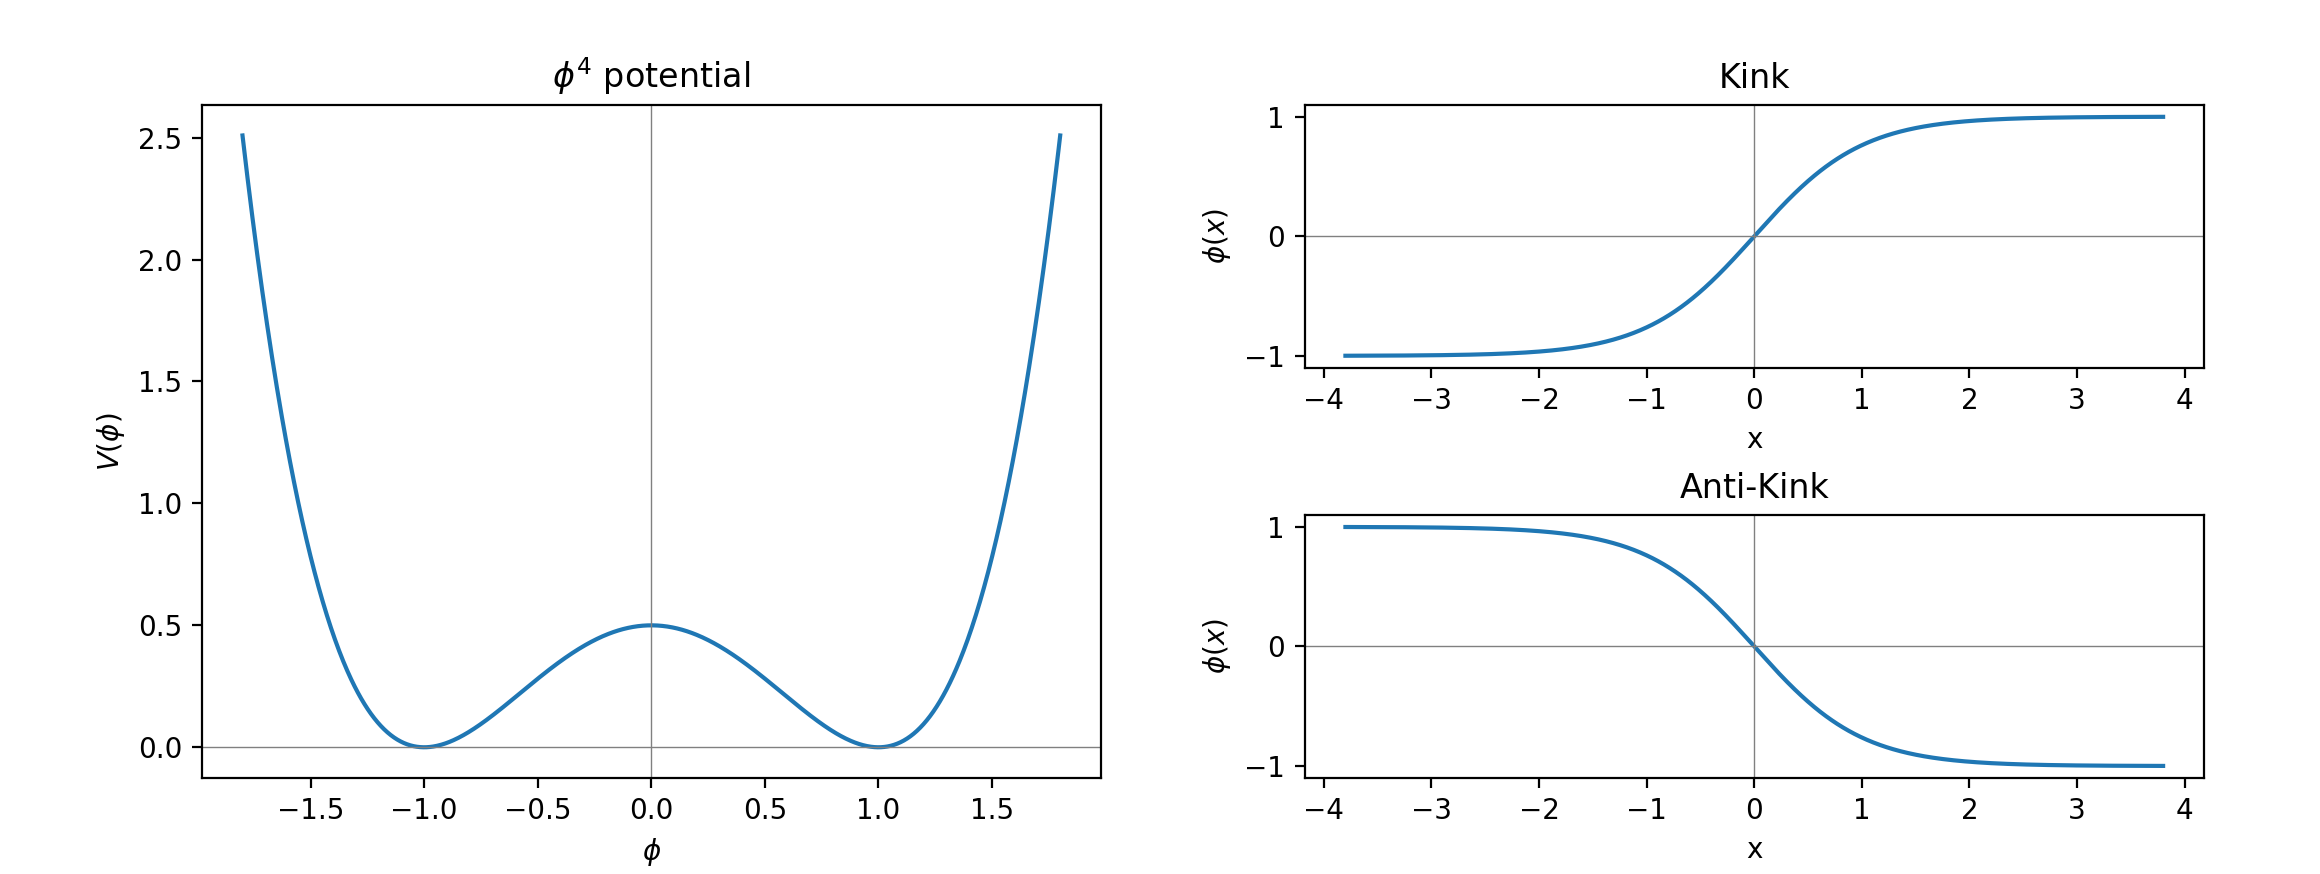
\includegraphics[width=0.8\textwidth]{phi4_potential.png}
 \captionof{figure}{Potential and kink shapes in $\phi^4$ theory} \label{phi4pot}
\end{figure}
Kink solutions emerge when the potential has a degenerate set of global minima. Since the dynamics of the system are unaffected by transformations of the form $V(\phi)\rightarrow V(\phi) + c$ for any constant $c$, we may assume that the minima of the potential occur at a set of field values $\phi_n \in \Phi_{\textup{vac}}$, where $V(\phi_n) = 0$. Each minimum of the energy implies the existence a vacuum solution to the field equation consisting of a static flat field where $\phi(x) = \phi_n$ across all of spacetime. If the field is in one vacuum state as $x\rightarrow -\infty$ and a different vacuum as $x\rightarrow \infty$ then a kink appears as the field must interpolate between the two minima over some region of spacetime. This kink is topologically protected, since to remove the kink one would need to shift an infinite length of field from one vacuum into another, costing an infinite amount of energy. By organising the minima in order of increasing $\phi$, we can label kink solutions as interpolating from $\phi_n$ to $\phi_{n+1}$ as $x$ goes from $-\infty \rightarrow \infty$ and anti-kink solutions as going from $\phi_n$ to $\phi_{n-1}$.\par
 The simplest example of such a potential is $\phi^4$ theory, described by $V_{\phi^4} = \frac{1}{2} (1-\phi^2)^2$. This has a minimum at $\phi_{-} = -1$ and at $\phi_{+} = +1$ as shown in fig.~\ref{phi4pot}. It can be shown that kinks take the form $\phi(x) = \tanh(x)$, see \cite{manton-book}.\par
 \begin{wrapfigure}{r}{0.45\textwidth}
\vspace{-10pt}
\centering
 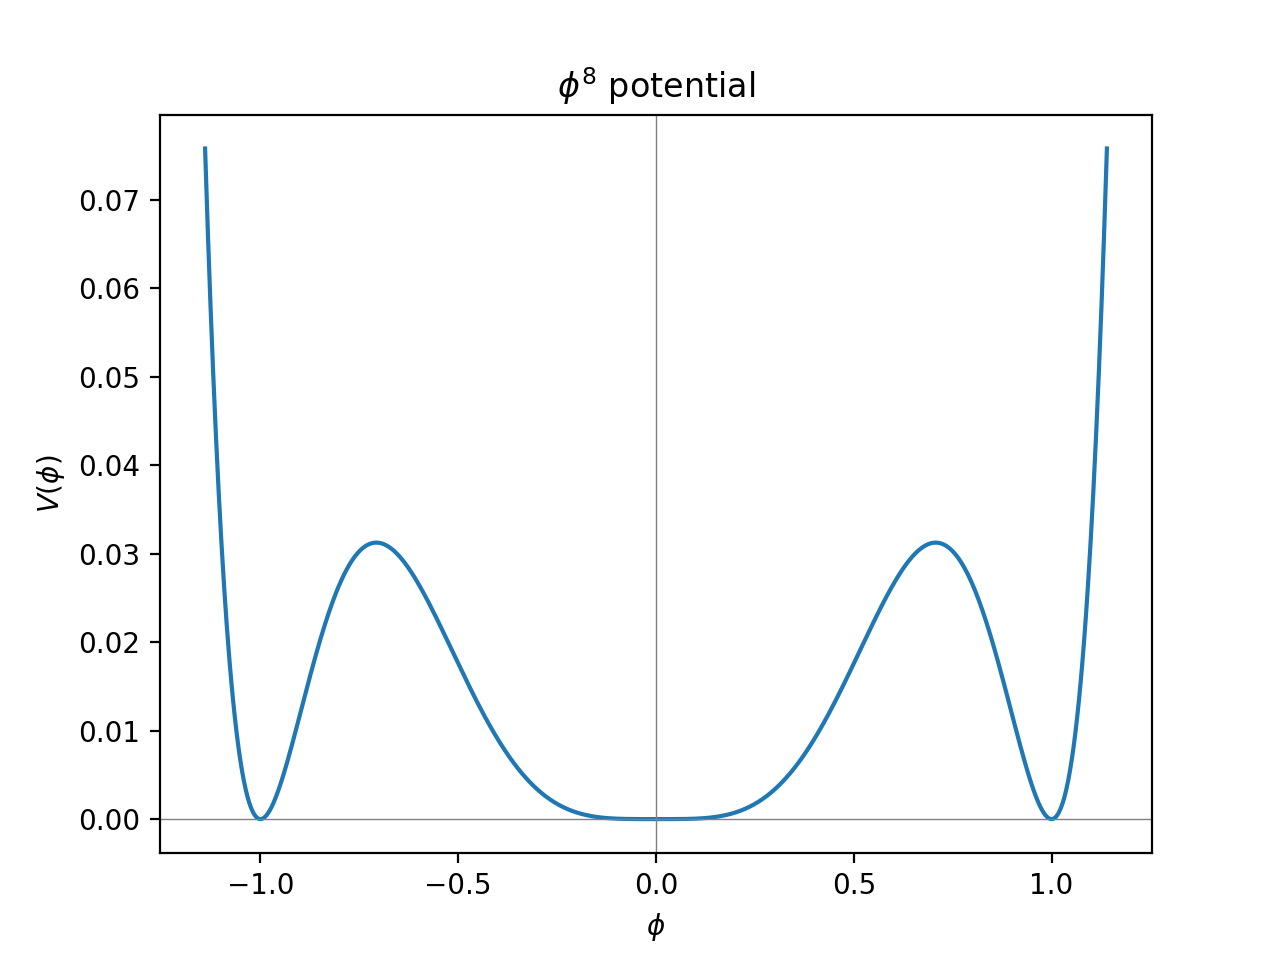
\includegraphics[width=0.45\textwidth]{phi8_potential.png}
 \captionof{figure}{Potential in $\phi^8$ theory} \label{phi8pot}
\end{wrapfigure}
 In this work we shall focus on kinks that emerge in the $\phi^8$ potential $V(\phi) = \frac{1}{2} \left ( 1 - \phi^2\right)^2 \phi^4$. The potential has three minima, a pair of quadratic minima at $\phi = \pm1$ and a quartic minimum at $\phi= 0$. We will label kinks as interpolating between $\phi = 0 \rightarrow 1$. Anti-kinks go from $\phi = 1 \rightarrow 0$, mirror kinks from $\phi = -1 \rightarrow 0$ and anti-mirror-kinks from $\phi = 0\rightarrow -1$. This potential is plotted in fig.~\ref{phi8pot}. It is worth noting that for small deviations around the quartic minimum, the potential is approximately flat, whereas around the quadratic minima the potential is quadratic. This means that the field around $\phi = 0$ appears massless, whereas around $\phi = \pm1$ it is massive. Throughout this essay we will refer to the field around the $\phi = 0$ vacuum as the massless field and that around $\phi = \pm1$ as the massive field. We elaborate on this further in \textsection \ref{kink_radiation}.\par
 Our first task is to derive the form of the kink appearing in this theory, using the Bogomolny trick \cite{bogomolny}. The kink is a static solution to the EOM (eqn.~\ref{EOM}). This means that the time derivative may be discarded, resulting in the following nonlinear ODE:
 \begin{equation} \label{kink_equation}
 {\phi}'' - \frac{\partial V}{\partial \phi} = 0, \textup{ with } V = \frac{1}{2} \left ( 1 - \phi^2\right)^2 \phi^4.
 \end{equation}
 This potential may be re-expressed in terms of a superpotential $W$ according to
 \begin{equation}
 V = \frac{1}{2} \left ( \frac{\textup{d}W}{\textup{d}\phi}\right )^2
 \end{equation}
 with
 \begin{equation}\label{dw}
 \frac{\textup{d}W}{\textup{d}\phi} = \left ( 1 - \phi^2 \right ) \phi^2 ,\; \;W = \frac{1}{3}\phi^3 - \frac{1}{5}\phi^5 +c.
 \end{equation}
For the sake of later convenience we shall set c to be $-\frac{2}{15}$, so that $W[1]=0$. We expect the kink solution to have $\phi_k (-\infty )= 0$ and $\phi_k (\infty )= 1$. Furthermore, the solution should be a minimum of the energy. Using the expression for energy density obtained in eqn.~\ref{energy}, we can write the total energy of the field as
 \begin{equation}\label{EW}
E = \frac{1}{2} \int_{-\infty}^{\infty} \left [ \left(\frac{\textup{d}\phi}{\textup{d}x}\right)^2 + \left(\frac{\textup{d}W}{\textup{d}\phi}\right)^2 \right ]\drv x.
 \end{equation}
 This may be rearranged by completing the square to give two equivalent expressions, depending on sign,
 \begin{equation}\label{energy_bogo}
E = \frac{1}{2} \int_{-\infty}^{\infty}\left (  \frac{\textup{d}\phi}{\textup{d}x} \mp \frac{\textup{d}W}{\textup{d}\phi} \right )^2 \drv x  \, \pm \left( W\left [  \phi(\infty)\right ]  -  W\left [  \phi(-\infty)\right ]\right).
 \end{equation}
$\phi(\pm\infty)$ will always be an element of $\Phi_{\textup{vac}} = \left \{ -1,0,+1\right \}$. From our expression for $W$ it can be shown that $W[-1] = -\frac{4}{15}$, $W[0] = -\frac{2}{15}$ and $W[1] = 0$.\par
 Equation \ref{EW} is a sum of two squares, so $E\geqslant 0$. This means that we should pick the sign to ensure that $ \pm \left( W\left [  \phi(\infty)\right ]  -  W\left [  \phi(-\infty)\right ]\right) \geqslant 0$ for our choice of limits. In the case of the kink, $\phi(-\infty) = 0,\, \phi(\infty) = 1 $, therefore $W\left [  \phi(\infty)\right ]  -  W\left [  \phi(-\infty)\right ] = \frac{2}{15}$ and so we pick the expression for the energy with a minus sign inside the integral. The total energy is minimised when the expression in the integral is 0, that is when
 \begin{equation}\label{bogo}
 \frac{\textup{d}\phi}{\textup{d}x} - \frac{\textup{d}W}{\textup{d}\phi} = 0.
 \end{equation}
 This equation is called the Bogomolny equation. Using eqn.~\ref{dw} this can be rearranged to give
 \begin{equation}
 \int \frac{\drv\phi}{\left(1-\phi^2 \right ) \phi^2} = \int \drv x
 \end{equation}
 which may be separated using partial fractions into
 \begin{equation}
 \int\drv\phi \left (\frac{1}{2\left(1+\phi\right )} + \frac{1}{2\left(1-\phi\right )} + \frac{1}{\phi^2} \right) = x -A
 \end{equation}
 and integrated to give an implicit expression for the shape of a kink
 \begin{equation}\label{long_kink_eq}
 x-A = \frac{1}{2}\log\left (\frac{1+\phi}{1-\phi} \right ) - \frac{1}{\phi}.
 \end{equation}
 Here the parameter $A$ may be interpreted as determining the position of the kink. This expression must be numerically inverted to give the form of the kink, shown in fig.~\ref{phi8kink}, as there is no explicit expression for the inverted kink profile $\phi_\textup{kink}(x)$. It is instructive to examine the asymptotic behaviour of the kink for $\phi$ close to 0 and close to 1. \par
  \begin{wrapfigure}{r}{0.45\textwidth}
\centering
 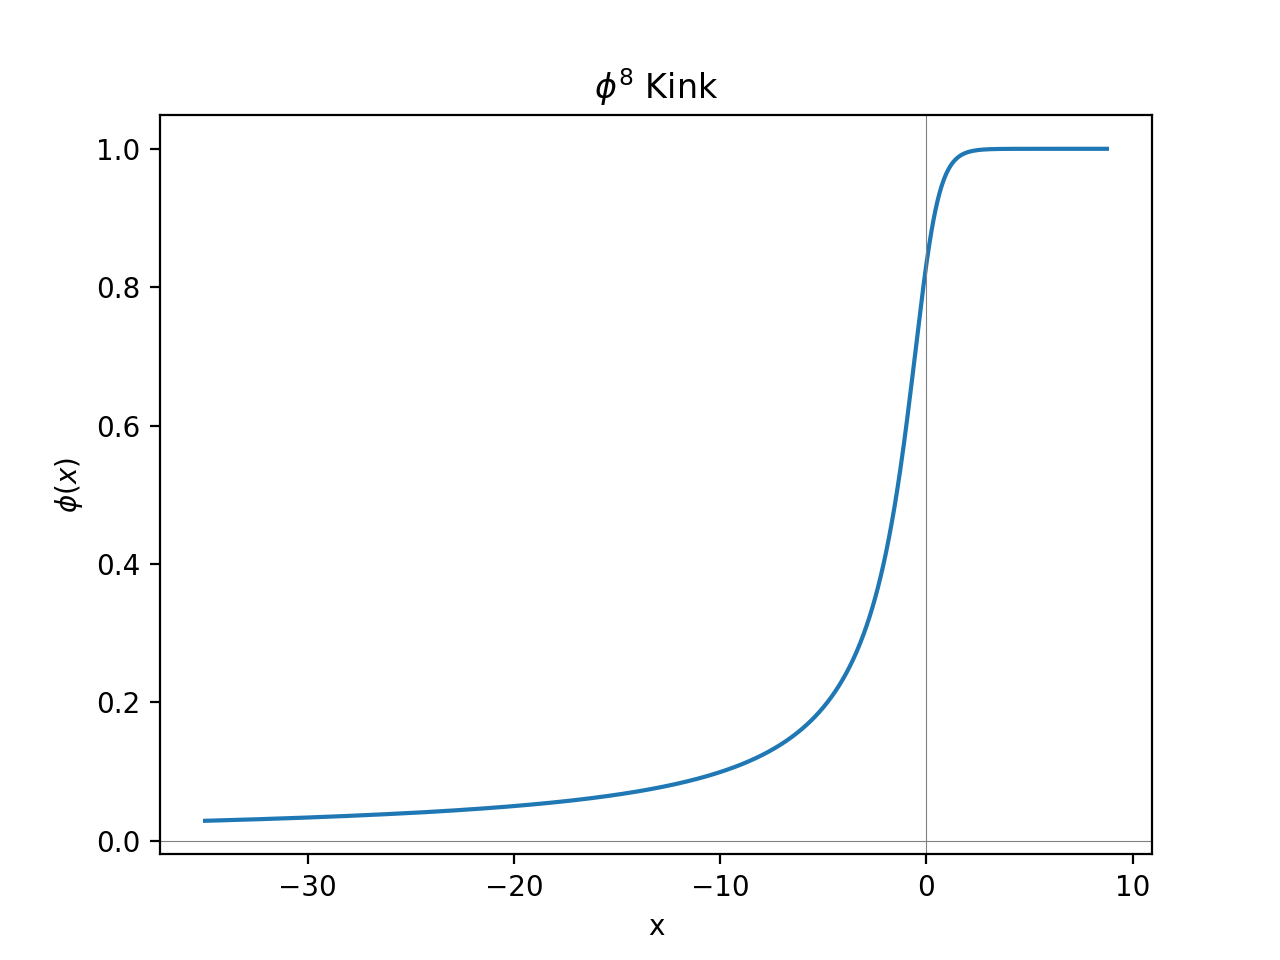
\includegraphics[width=0.45\textwidth]{phi8_kink.png}
 \captionof{figure}{Kink in $\phi^8$ theory} \label{phi8kink}
\end{wrapfigure}
 On the left hand side of the kink, $\phi = \epsilon$ with $\epsilon$ small and positive. In this case, eqn.~\ref{bogo} reduces to $\frac{\drv \epsilon}{\drv x} = \epsilon^2$, which can be solved to give 
 \begin{equation}
 \phi_\textup{left} = \frac{1}{A-x}.
 \end{equation}
 On the right hand side $\phi = 1- \epsilon$ with $\epsilon$ small and positive and eqn.~\ref{long_kink_eq} can be expanded to first order to give
 \begin{equation}
 \frac{1}{2} \log2 - \frac{1}{2} \log \epsilon - 1 = x-A
 \end{equation}
 which gives the following expression for $\phi_{\textup{right}}$
 \begin{equation}
 \phi_{\textup{right}} = 1- \exp\left [ -2\left ( x - A + 1 - \frac{1}{2}\log2 \right ) \right ].
 \end{equation}
 In the case of $\phi^4$ theory, the field decays exponentially quickly on both sides to the minima of the potential. However in the case of $\phi^8$ theory, the decay on the left of the kink has an extremely long tail, allowing for long range interactions.\par
 Here it is worth mentioning the mechanical reinterpretation of the kink solution, since it will be useful later on. Equation \ref{kink_equation} may be interpreted as the equation of motion for a particle with `position' $\phi$ moving in a potential $-V(\phi)$. To produce a kink, the particle starts at $\phi = 0$, the maximum of the potential, with infinitesimal positive velocity. It moves quickly through the trough and then slows town to asymptotically approach the next maximum at $\phi = 1$. Since energy is conserved in this system (there is no drag term) the particle will come to rest at the next maximum, at the same value of potential the particle started with. This is shown in fig.~\ref{mech}. As the `particle' moves, it sweeps out the profile of the kink.\par
 \begin{wrapfigure}{L}{0.45\textwidth}
 \vspace{-10pt}
\centering
 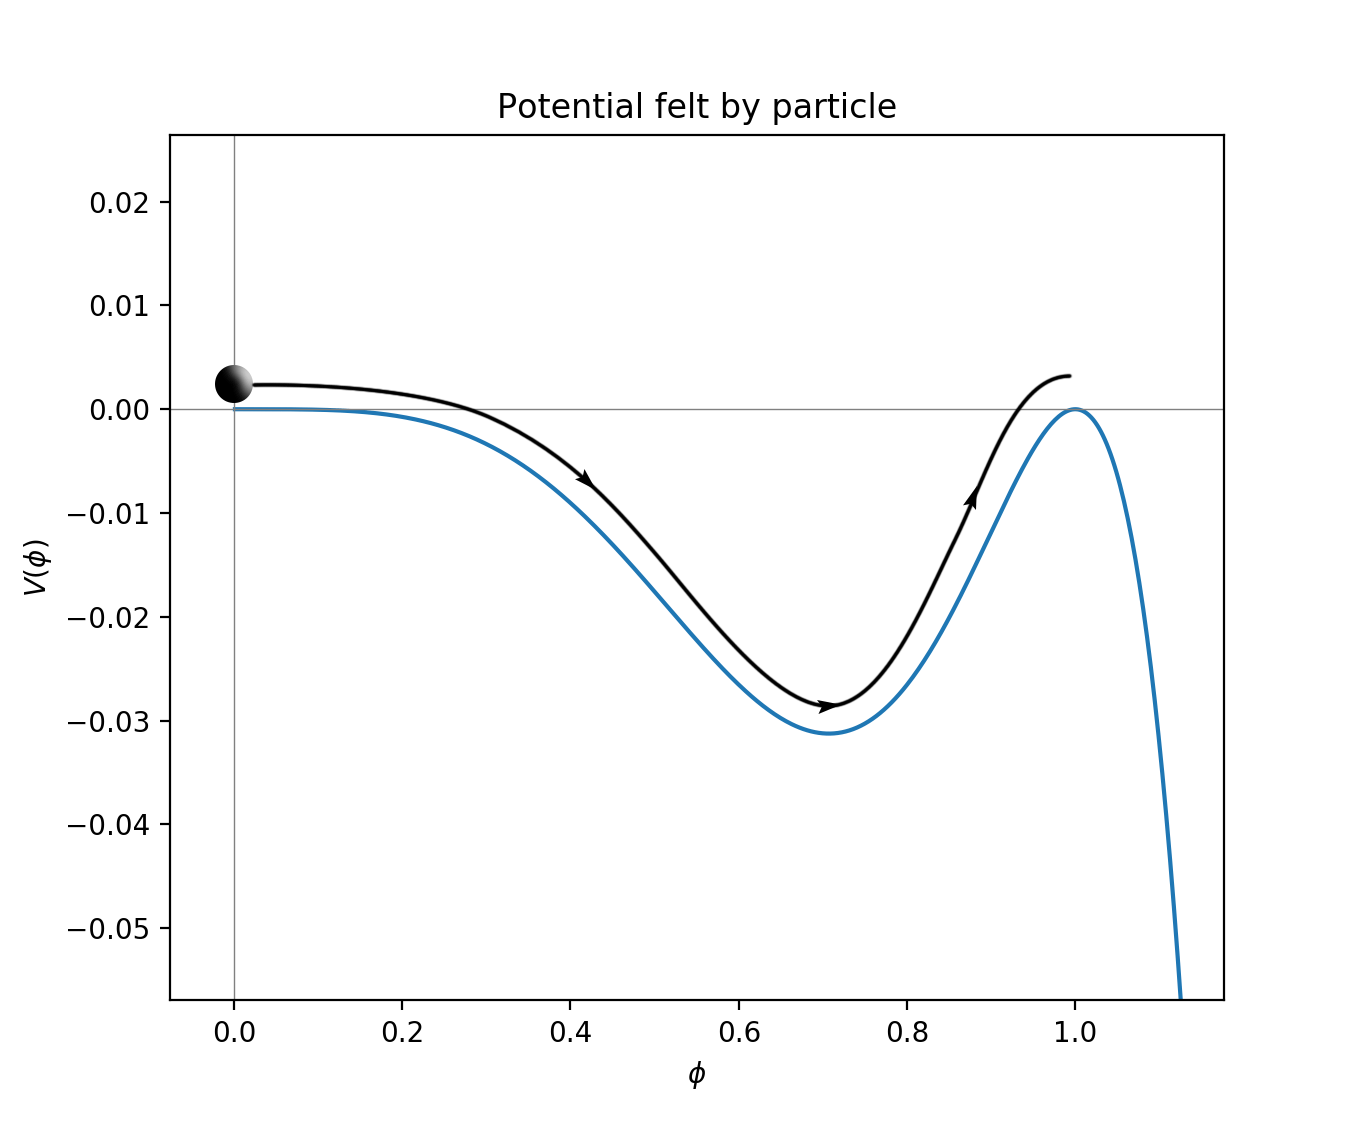
\includegraphics[width=0.45\textwidth]{mech_kink.png}
 \captionof{figure}{Inverted potential felt by the particle in the mechanical reinterpretation} \label{mech}
 \vspace{-23pt}
\end{wrapfigure} 
 Finally we discuss the mass of the kink. From eqn.~\ref{energy_bogo} we can see that, once the Bogomolny equation is satisfied, the total energy of a kink is $2/15$. Thus, since the theory is Lorentz invariant, the kink may be interpreted as a particle-like object with mass = 2/15. Furthermore, since the Bogomolny equation is satisfied locally at every point in space, the total energy of the field between two points $x_1$ and $x_2$ can be calculated as $\left | W\left [ \phi(x_1)\right ] - W\left [ \phi(x_2)\right ]\right |$.
 
 \section{Kink-Kink Interactions}
 We now turn our attention to modelling the force between a well-separated kink and anti-kink. In all cases the kinks are ordered such that the interaction is due to overlapping of their long range $\frac{1}{x}$ tails. The short-range tail on the other side has exponential asymptotics so interactions where these tails overlap will be largely identical to those in $\phi^4$ theory and we do not study them here. The force is initially calculated analytically by approximately deriving a profile for the field. By examining the momentum density of the field, it is possible to extract the force acting on the pair. The analytical discussion here follows \cite{manton-paper}. In \textsection \ref{kink_kink_comp} the results are numerically simulated.\par


\subsection{Analytic Model}\label{kink-kink-analytic}
  \begin{wrapfigure}{R}{0.5\textwidth}
  \vspace{-10pt}
\centering
 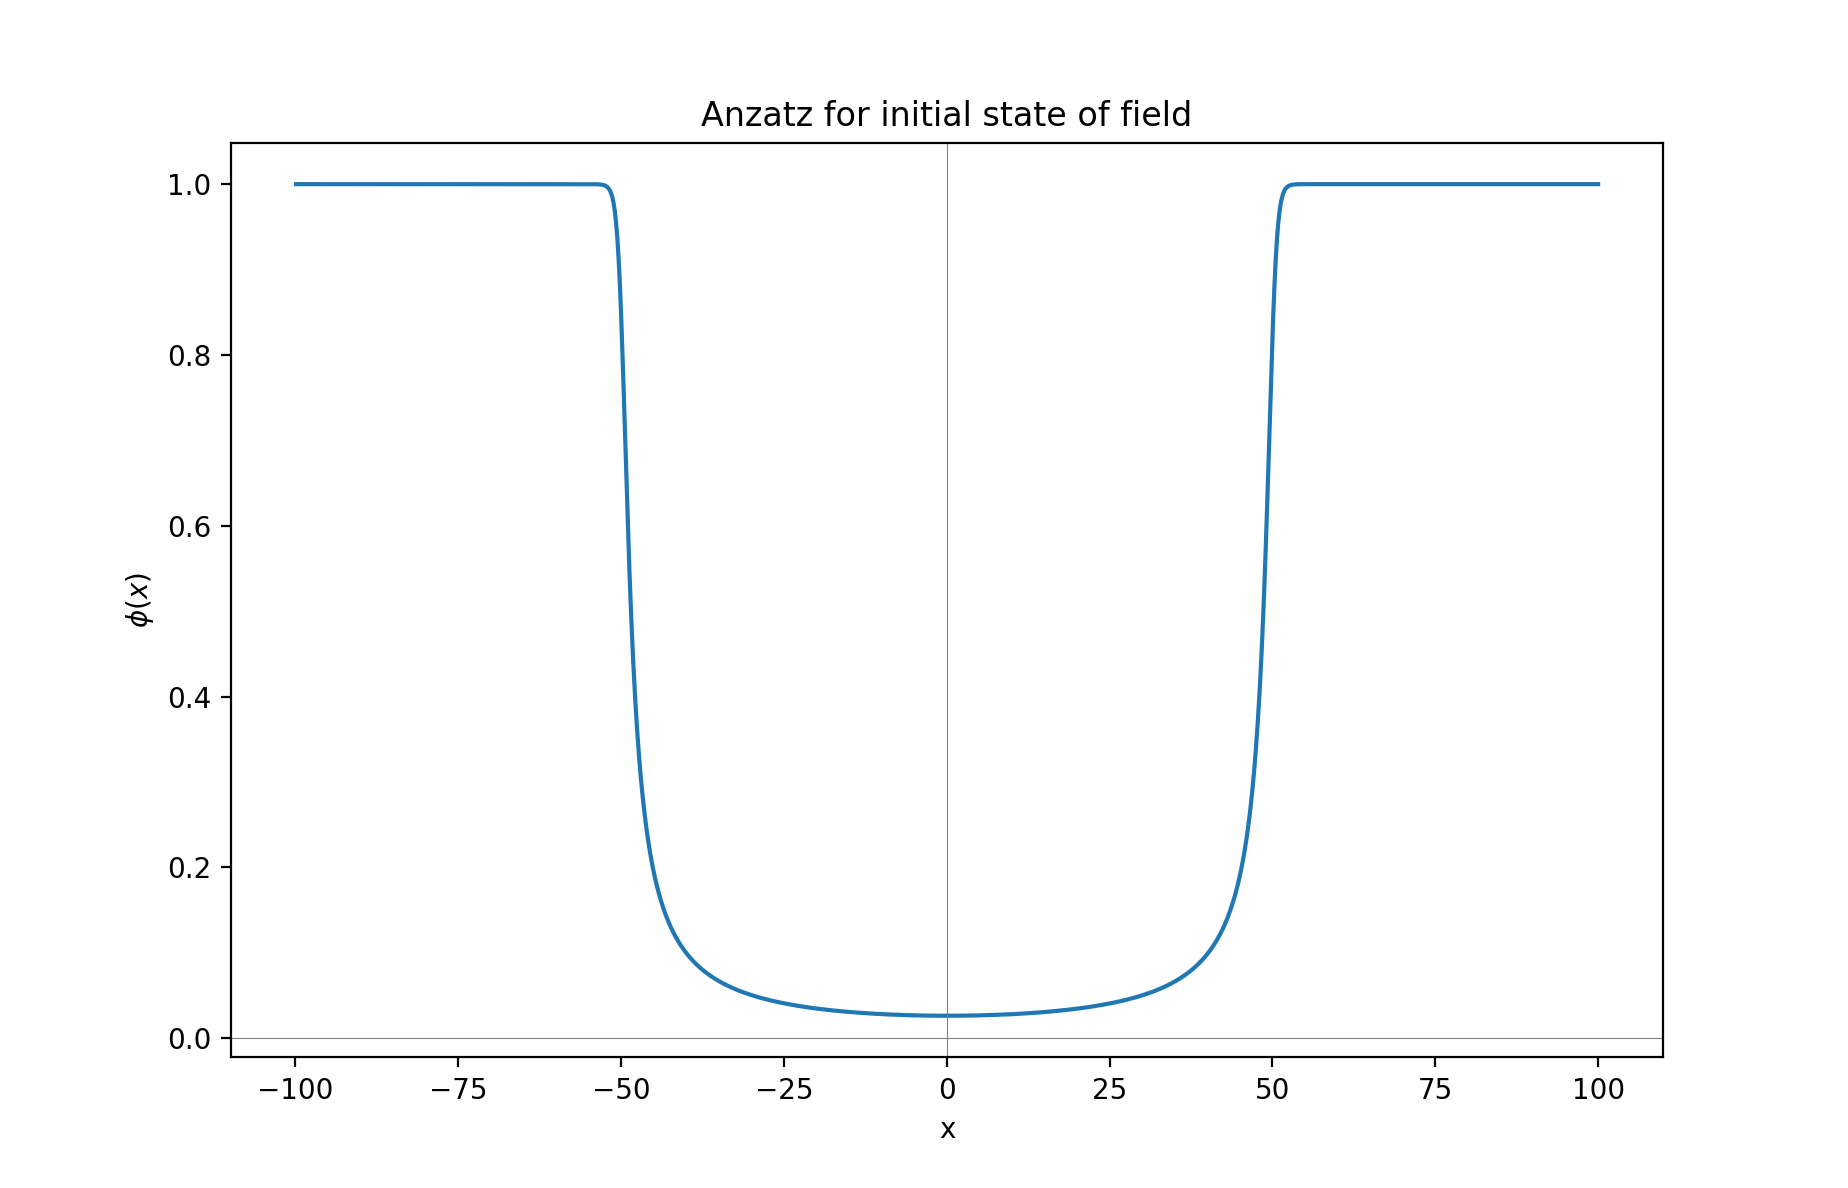
\includegraphics[width=0.5\textwidth]{kink-kink_init.png}
 \captionof{figure}{A possible state containing a kink and anti-kink} \label{kink_kink_state}
 \vspace{-10pt}
\end{wrapfigure} 
To calculate the force between an interacting kink and anti-kink pair, we must make a guess at an appropriate field containing these two objects. In particular, since the system we are looking at is no longer static - the kinks are accelerating towards one another - it will be necessary to account for the distortion of the kink profile caused by this acceleration. Let us start with a field in which the anti-kink is at position $-A(t)$, the kink is at $A(t)$ and the field is initially at rest.\par
The kink and anti-kink have identical form, but reflected over the y-axis, therefore it is reasonable to propose a configuration that is symmetric over the y-axis, as shown in fig.~\ref{kink_kink_state}. Here the anti-kink is positioned at $x = -50$ and the kink is at $x= 50$. Note that the field between the kinks should not touch the x-axis. Additionally, the field will be distorted from the static kink solution, with $\phi' = 0$ at $x=0$.\par
Such a field may be approximated by looking for a solution to the field equation for an accelerating kink (i.e. where $\ddot{A}(t) = a$). The tail of this kink will be distorted from the static solution, having $\phi' = 0$ at some distance from the kink. Thus we may glue the tails of an accelerating kink and anti-kink together at $x=0$. The acceleration of the anti-kink will be $a$, so the acceleration of our field will jump discontinuously as we cross $x=0$, from $a$ to $-a$, therefore this solution will not be exact, but rather a good approximation. \par
Before calculating the shape of this field, we first examine how the force acting on a kink may be determined from the field configuration. From eqn.~\ref{momentum} it can be seen that the momentum density is given by $\mathcal{P} = -\dot{\phi}\phi'$. Therefore, the rate of change of the total momentum in a region from $x_a$ to $x_b$ is given by
\begin{align}
\frac{\drv P}{\drv t} &= -\frac{\drv}{\drv t} \int_{x_a}^{x_b} \dot{\phi}\phi' \drv x \\
 &= - \int_{x_a}^{x_b} \left ( \ddot{\phi}\phi' + \dot{\phi}\dot{\phi'} \right )\drv x.
\end{align}
From the equations of motion, $\ddot{\phi} = \phi'' - \frac{\drv V}{\drv\phi}$, the expression becomes
 \begin{equation}
\frac{\drv P}{\drv t} = - \int_{x_a}^{x_b} \left ( \phi'' \phi' - \frac{\drv V}{\drv\phi} \phi' + \dot{\phi}\dot{\phi'} \right )\drv x
\end{equation}
which may be integrated to give an expression for the force acting on the region between $x_a$ and $x_b$
\begin{equation}
F = -\left [ \frac{1}{2} \phi'^2 + \frac{1}{2} \dot{\phi}^2 - V(\phi) \right ]_{x_a}^{x_b}.
 \end{equation}
 In the case of two interacting kinks shown in fig.~\ref{kink_kink_state}, the force acting on the kink can be determined by setting $x_a = 0$ and $x_b = \infty$. The field at $ x =\infty$ is in the ground state and does not contribute to the force. We expect the field at $x=0$ to have no spatial first derivative and negligible time derivative, since the field starts from rest and is initially slow moving. Thus we are left with only one contributing term
 \begin{equation} \label{force}
F_\textup{kink} = - V[\phi(0)].
 \end{equation}
 This means that, when calculating an approximate profile for the kink-anti-kink interaction, it is most important to ensure that the field is accurate in the region around $x=0$.\par
 Now we return to determining a form for the field of an accelerating kink. The first step is to model the kink with an expression of the form
 \begin{equation}
 \phi(x,t) = \chi\left( x - A(t)\right).
 \end{equation}
 This can also be written as $\chi\left( y\right)$ for $y = x-A(t)$. Substituting into the equations of motion gives
 \begin{equation}
 \chi '' \dot{A}^2 - \chi'\ddot{A} - \chi '' + \frac{\drv V }{\drv \chi}=0.
 \end{equation}
 We are starting with a field at rest so the expectation is that $\dot{A}$ is small and so the term $\chi '' \dot{A}^2$ may be ignored. Additionally, we set $\ddot{A} = -a$, ending up with
 \begin{equation} \label{acc_kink}
 \chi'' - a\chi' - \frac{\drv V }{\drv \chi}=0.
 \end{equation}
In the mechanical interpretation, this may be understood as describing the dynamics of a particle moving in the same potential as fig.~\ref{mech}, but with a negative drag term, $-a$. The effect of $a$ is to add energy to the system as the particle moves under the influence of $V(\chi)$. The solution we are looking for corresponds to the particle starting from rest ($\chi' = 0$) at a point $\chi >0$ and gaining just enough energy over its motion to make it to the top of the maximum in potential at $\chi=1$, where it returns asymptotically to rest. For each value of $a$ there is a position $\chi(0)$ such that a particle starting at that point and moving under drag $-a$ will gain just enough energy to reach the maximum at $\chi=1$ and go no further, resulting in a valid kink solution. This will correspond to a kink that starts at a finite $\chi(0)>0$, with flat gradient, $\chi'(0)=0$ and tends to $\chi=1$ as $x \rightarrow \infty$.\par
In what follows, we assume that the majority of the influence of the drag term is exerted on the long-range tail of the kink. This makes sense since the tail is extremely long. The drag force is weaker in the tail region than it is around the centre of the kink, but not substantially so, and acts over a much larger region. To compare the accelerating kink with the static kink derived in \textsection \ref{set_scene} we match the shapes of the long tails of both, in particular, aligning them so that the extrapolation of their $\frac{1}{x}$ tails diverge at the same point. This is shown in fig.~\ref{tails}, where the point at which the tail diverges is marked with a dashed line.\par
\begin{figure}
\centering
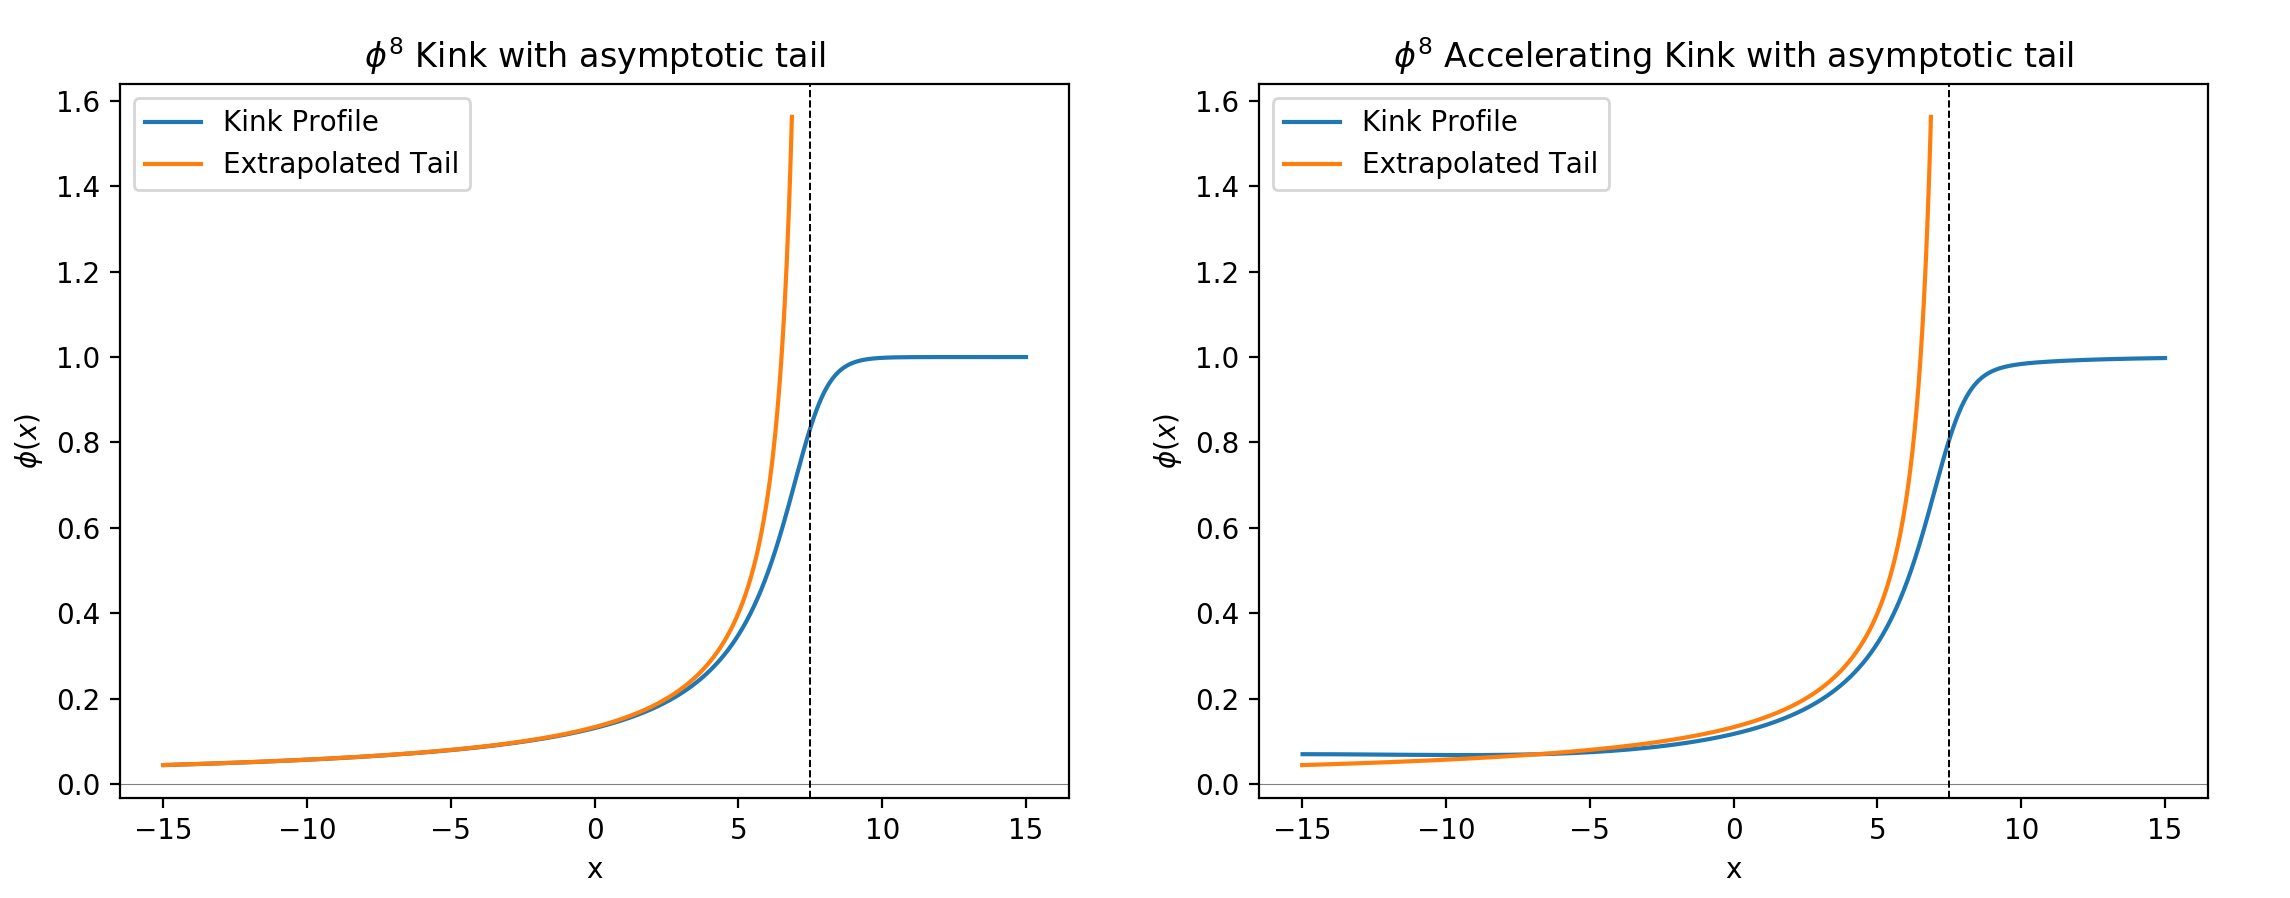
\includegraphics[width=0.9\textwidth]{asym_tails.png}
\captionof{figure}{Static and accelerating kink with extrapolated tail behaviour. The points at which the extrapolated tails diverge are marked with a dashed line.} \label{tails}
\end{figure}
We can assume that $\chi$ approximately takes the form of an undeformed kink over its long tail, ensuring that it is a solution of the Bogomolny equation ($\chi' = \frac{\drv W }{\drv \chi}$), with $W$ defined in eqn.~\ref{dw}. Thus, eqn.~\ref{acc_kink} becomes
\begin{equation}\label{VW}
\chi'' -\frac{\drv}{\drv \chi}\left ( aW + V \right ) =0.
\end{equation}
We can now define a modified potential $\tilde{V} = V +aW$ and integrate eqn.~\ref{VW}.
\begin{equation}
\int \chi'' \chi' \drv x = \int \frac{\drv \tilde{V}}{\drv \chi} \drv \chi
\end{equation}
to get
\begin{equation}
\chi'^{\,2} = 2 \tilde{V}.
\end{equation}
In the long-tail region, $\chi$ is small, so $V\simeq \frac{1}{2}\chi^4$ and $W\simeq -\frac{2}{15}$, thus we obtain
\begin{equation}\label{chi_prime}
\chi' = \sqrt{\chi^4 - \frac{4a}{15}}.
\end{equation}
$\chi$ takes its smallest value at $x=0$ where $\frac{\drv\chi}{\drv x}=0$. Therefore for eqn.~\ref{chi_prime} to hold we must have $\chi(-A) = \left( \frac{4a}{15} \right)^{1/4}$ (where we used $y = x-A$). Note that from eqn.~\ref{force} this means that the force acting on the kink is given by
\begin{equation}
F = -V\left[\chi(0)\right] = -\frac{2a}{15}
\end{equation}
which is perfectly consistent with $F = ma$ for a kink of mass $\frac{2}{15}$ and acceleration $a$. We wish to fix the solution of eqn.~\ref{chi_prime} to ensure that it diverges at $x = A$, ($y = 0$), since the extrapolation of a static kink diverges at $x=A$. We therefore have $\chi(0) = \infty$. Having set our limits, we can integrate eqn.~\ref{chi_prime} to get
\begin{equation}
\int_{ \left( \frac{4a}{15} \right)^{\frac{1}{4}}}^{\infty}\frac{\drv \chi}{\sqrt{\chi^4 - \frac{4a}{15}}} = A.
\end{equation}
Making the substitution $\chi =\left( \frac{4a}{15}\right)^{\frac{1}{4}}\lambda$ gives
\begin{equation}
 \int_{1}^{\infty}\frac{\drv \chi}{\sqrt{\chi^4 - 1}} = \left( \frac{4a}{15}\right)^{\frac{1}{4}} A.
\end{equation}
Now, by making a further change of variables $\lambda^2 = \cosh\nu$ we get
\begin{equation}
 \left( \frac{4a}{15}\right)^{\frac{1}{4}} A = \frac{1}{2}\int_{0}^{\infty} (\cosh\nu)^{-1/2}\drv \nu
\end{equation}
which finally gives
\begin{equation}
 \left( \frac{4a}{15}\right)^{\frac{1}{4}} A =\frac{1}{\sqrt{2}}\frac{\Gamma \left( \frac{1}{4}\right)^2}{4\sqrt{\pi}}.
\end{equation}
Plugging this result into eqn.~\ref{force} and evaluating gives
\begin{equation} \label{prediction}
F \simeq -\frac{1.477}{A^4}.
\end{equation}

\subsection{Numerical Simulation of Interacting Kinks} \label{kink_kink_comp}
The result calculated in the previous section is now tested by numerically solving the equations of motion for an interacting kink and anti-kink. The primary difficulty once again is in making a good guess for the initial shape of a field containing the kink-anti-kink pair.\par
To simulate the field, we must numerically solve the partial differential equations of motion (eqn.~\ref{EOM}), given the initial state of the field and its derivative with respect to time, $\phi(x;t=0)$ and $\dot{\phi}(x;t=0)$. This is done by splitting up our region of space into $N_x$ discrete steps, in this case we used $N_x = 2048$\footnote{In later calculations we will calculate the discrete Fourier transform of the field. Setting the array to have a size $N_x = 2^k$ for an integer k will allow the discrete fourier transform to be calculated in $O(\log N_x)$ time, rather than $O(N_x^2)$, using the fast fourier transform algorithm, providing us with a substantial speedup.}. Thus, the field at time 0 becomes a 2048-entry array $\phi_i$. Spectral methods are used to approximate the spatial derivatives of $\phi_i$ in eqn.~\ref{EOM}, based on \cite{spectral}. This technique relies on creating an interpolating function for $\phi(x)$ from $\phi_i$, and outputting the derivatives of that function. The method is extremely accurate, but comes with two important limitations. The first is that results are highly sensitive to the smoothness of the input array. Any discontinuity in the array or its first few derivatives will lead to substantial inaccuracies. Secondly, the method only works in systems with periodic boundary conditions. It is possible to express the spectral differentiation operator as a matrix $D_{ij}$, and we will refer to it as such in equations written here, however in practice it is much faster to compute it using discrete Fourier transforms, which is the technique used in our calculations. In our case, we modelled the interacting kinks over a spatial distance $x_\textup{max} = 200$ with periodic boundary conditions. The PDE (eqn.~\ref{EOM}) may now be expressed in terms of the $N_x$ entries of an array $\phi_i(t)$ as a set of 2048 coupled nonlinear second-order ordinary differential equations:
\begin{figure}
\centering
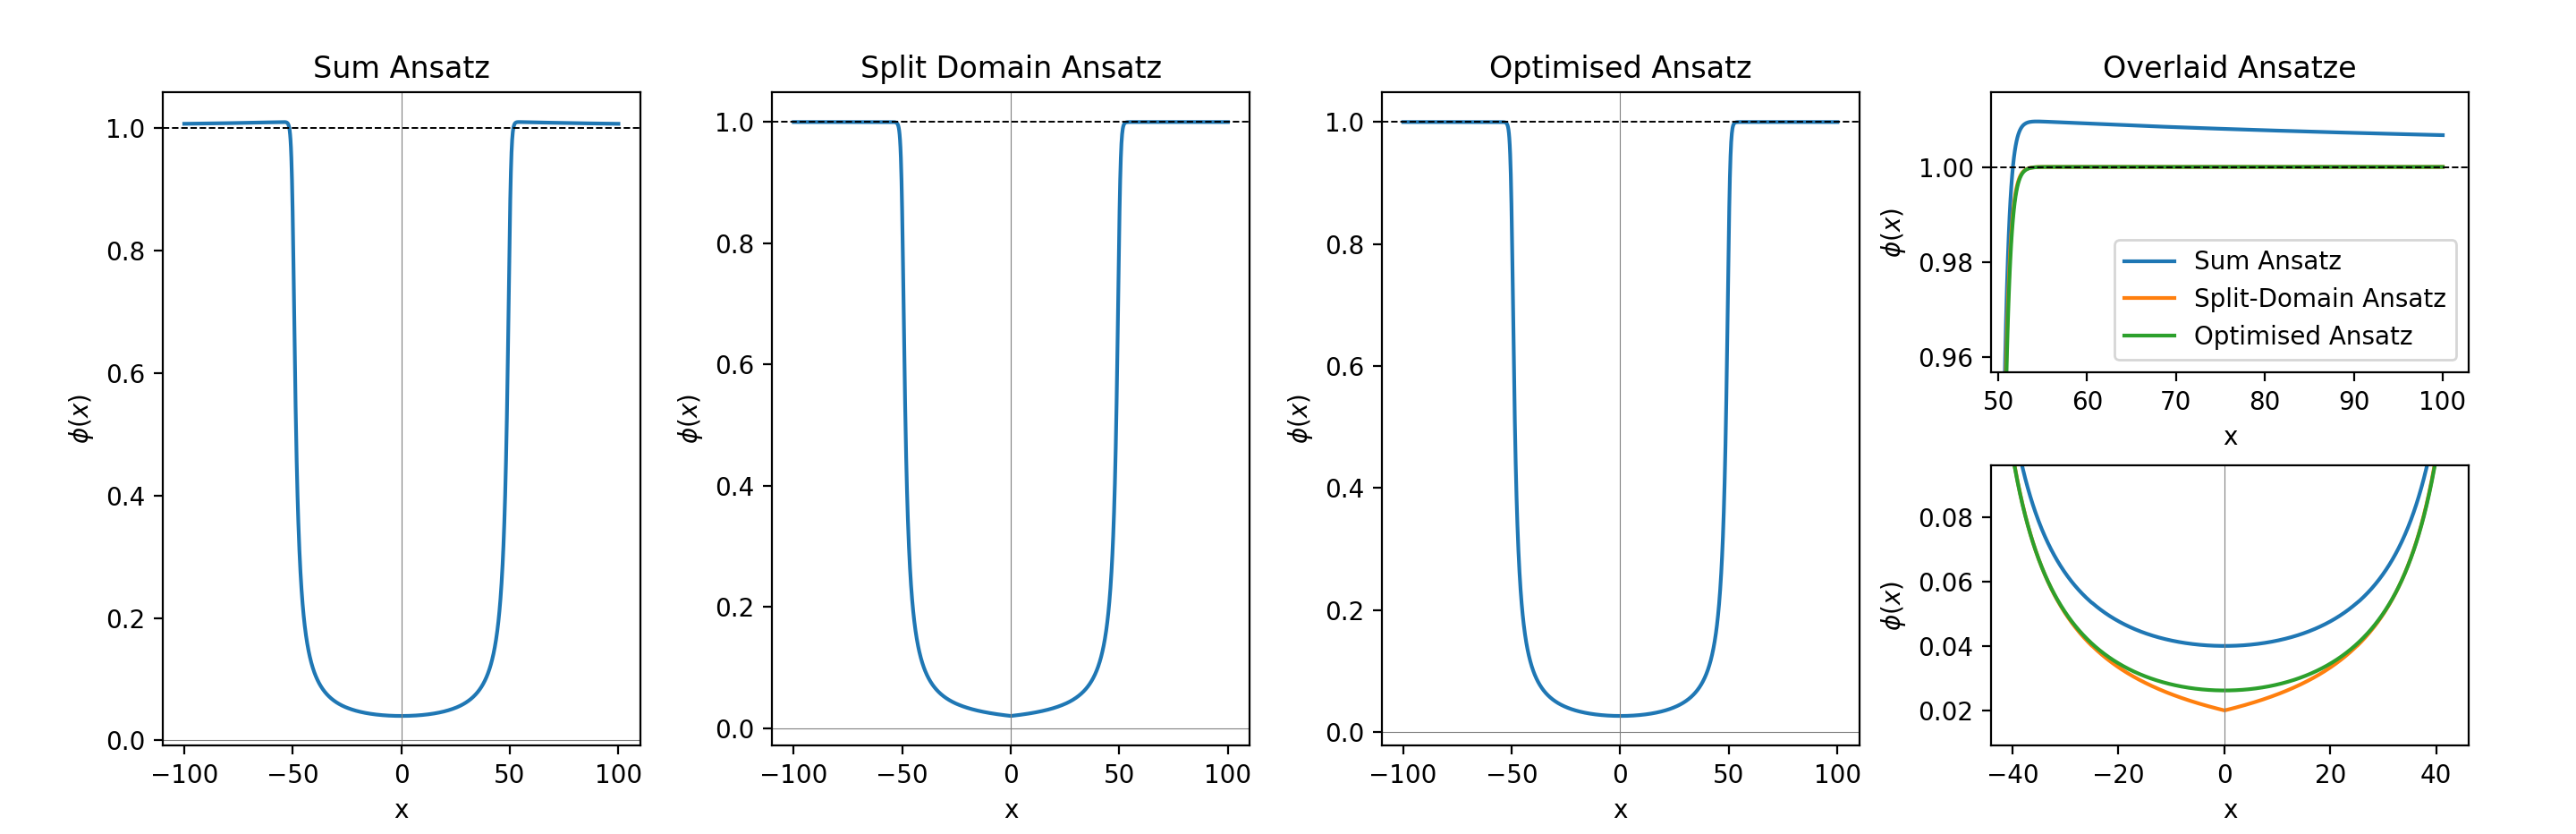
\includegraphics[width=\textwidth]{field_ansatze.png}
\captionof{figure}{Plots of the sum ansatz, split-domain ansatz and optimised ansatz. In the fourth graph it can be clearly seen that not only does the sum ansatz give the wrong shape at the edges, where the field should be sitting in the $\phi=1$ vacuum, but $\phi$ is far from the correct value even in the region between the kinks.}\label{ansatze}
\end{figure}
\begin{equation}
\ddot{\phi_i} - D^2_{ij}\phi_j + V'(\phi_i) = 0.
\end{equation}
Setting $\phi_i(t) = u_i(t)$ and $\dot{\phi_i}(t) = v_i(t)$ we can re-express this as a set of 4096 coupled first-order differential equations
\begin{align}
\dot{v_i} &= D^2_{ij}u_j - V'(u_i) \\
\dot{u_i} &= v_i .
\end{align}
 These equations can be solved in Python using the Scipy library's built-in ODE solver, \texttt{odeint}, as an initial value problem for a specified $u_{j}(0)$ and $v_{j}(0)$. Tests are conducted to verify the accuracy of this method, ensuring that the results obey momentum and energy-conservation. These are detailed in appendix \ref{tests}, confirming that the method works accurately.\par
 As in \textsection \ref{kink-kink-analytic}, the primary complication here is in choosing an appropriate starting configuration for the field containing an interacting kink and anti-kink. Due to the long-range nature of the kink's tail, it is not possible to sum the static field for a kink at position $A$ with that of an anti-kink at position $-A$. This is because the long range tails decay so slowly that they pass through the other kink to the side that should be exponentially decaying to the vacuum, disturbing the field from its vacuum value.\par
 Our approach closely follows that taken in \cite{christov-num}. The first step is to make a crude guess at the shape of the field. In this case we have used the split-domain ansatz, where the field for $x>0$ is taken as that of a kink at $x=A$, and the field at $x<0$ is that of an anti-kink at $x=-A$. The two fields are glued together at $x=0$, leaving a discontinuity in the first derivative.\par
 We are looking for the field that comes closest to approximately solving the static-field equations of motion, while still containing a kink at $A$ and an anti-kink at $-A$. Thus, we may improve our guess for the initial field using a weighted nonlinear least squares minimisation of the function
 \begin{equation}\label{optimise}
 \mathcal{I}[\phi] = \left \| D^2\phi -V'\left( \phi \right) \right \|^2 + C\left | \phi(A) - \phi_0 \right |^2 + C\left | \phi(-A) - \phi_0 \right |^2
 \end{equation}
 where $\phi_0$ is $\phi_{\textup{kink}}(x=0,A=0) \approx 0.8335$ and C is a sufficiently large number, we have taken $C = 50$. The first term here is the static part of the equations of motion, ensuring that the optimised field is close to a static solution. The second part ensures that the field has a kink at $A$ and an anti-kink at $-A$ by forcing the optimisation to keep $\phi$ close to $\phi_0$ at $x=A$ and $x=-A$. The optimised solution for $A=50$ is shown in fig.~\ref{ansatze}.\par
 Now that we have reliable methods in place to initialise our field values and propagate them forward in time, we are ready to calculate the force acting between a kink and anti-kink. Our first step is to initialise the fields for a number of values of $A$. Here we have chosen to look from $A=10$ to $A = 90$, stepping up in intervals of 5. After optimisation, using eqn.~\ref{optimise}, the fields are evolved in time from $t=0$ to $t=1000$. Figure \ref{field_evolutions} shows the results for $A =$20, 30 and 70. Full results can be found at https://github.com/dpreuo/Kinks-with-Long-range-interactions.\par
 \begin{figure}
\centering
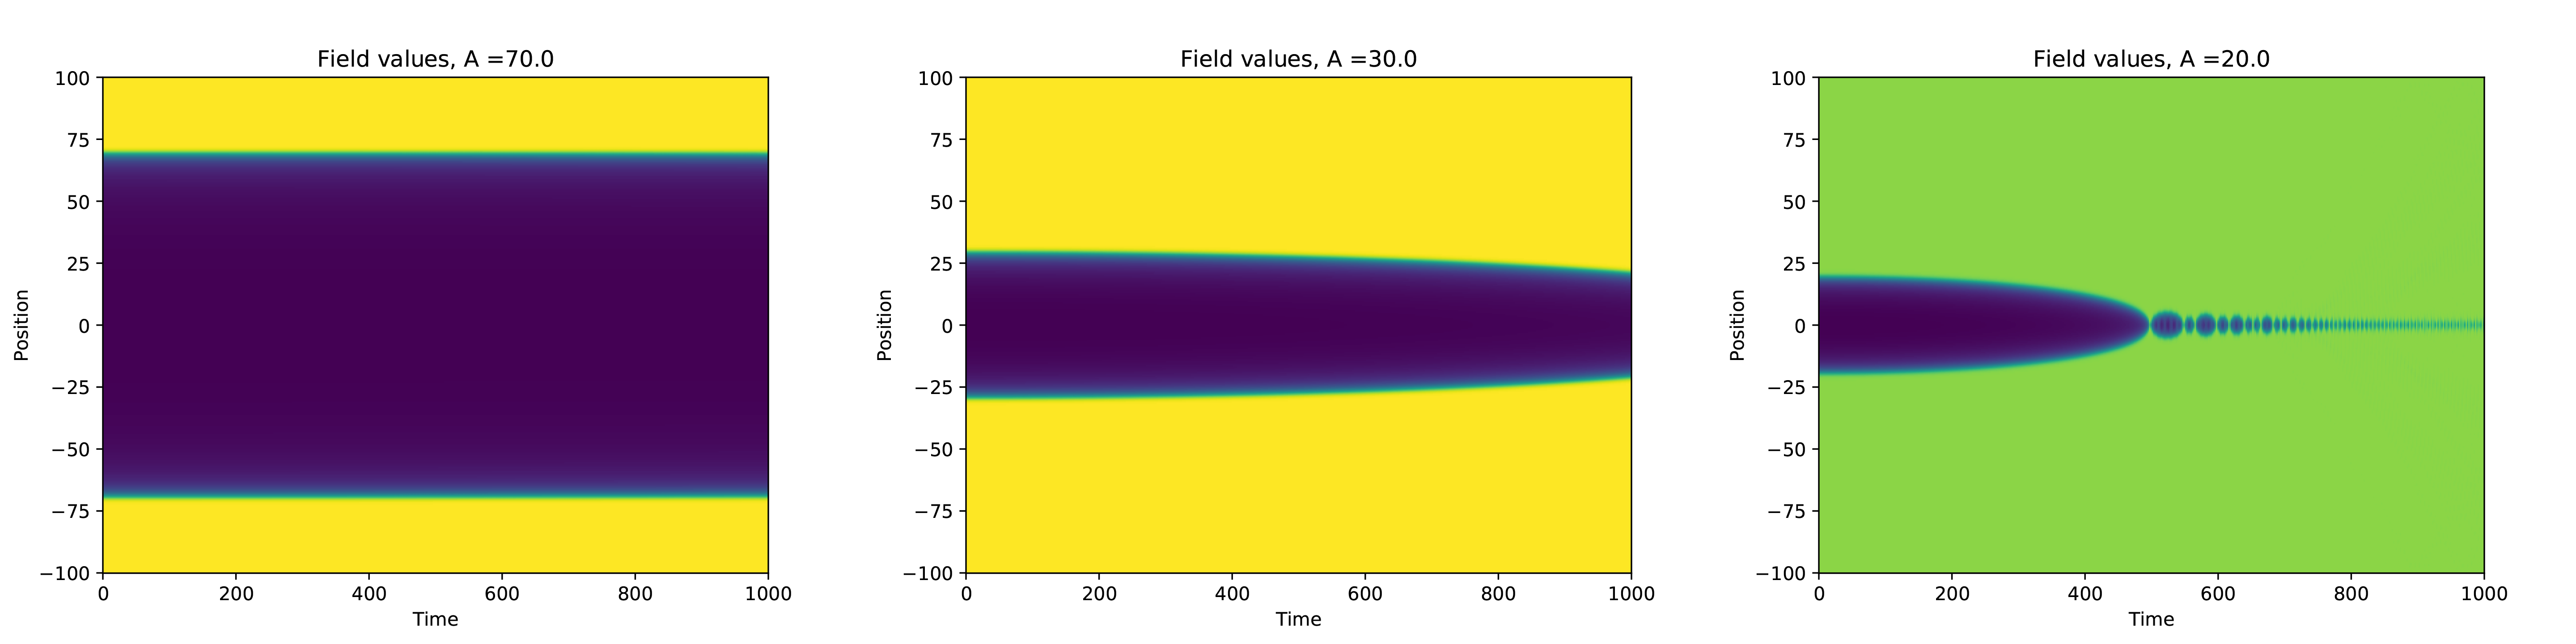
\includegraphics[width=\textwidth]{field_values}
\captionof{figure}{Plots of field values against time. In the first plot, the kinks start extremely far apart, at $A=70$ and their acceleration towards one another is not noticeable. For $A = 30$ one can see their acceleration towards one another. Finally when they start at $A=20$, they collide at $t\approx450$ creating an oscillon that gradually decays into radiation.} \label{field_evolutions}
\end{figure}
Now, the momentum density of the field is calculated using eqn.~\ref{momentum}. We can compute the total momenta of the kink and anti-kink by integrating the momentum density over the spatial regions $x>0$ and $x<0$ for each point in time. Then $F = \frac{\drv P}{\drv t}$ is calculated for the kink and anti-kink by approximating the derivative using second order finite difference methods. In order to compare this to our analytic prediction, we calculate the position of the kink as a function of time and multiply it with $F$. From eqn.~\ref{prediction} we can see that the expected result is
\begin{equation}
F(t) A^4(t) =\frac{1}{4} \left (\frac{ \Gamma\left(\frac{1}{4}\right)^2}{4\sqrt{2\pi} }\right )^4 \approx 1.47713.
\end{equation}
Figure \ref{force_graphs} shows the results for $FA^4$ as a function of time for starting values of $A(0) = $ 25, 50 and 65. There are small disturbances of order $10^{-2}$, caused by imperfections in the optimisation of the initial conditions producing radiation and other deviations from the ideal starting field that then interfere with the motion of the kinks. However despite this it can clearly be seen that the majority of the graph is approximately flat, confirming the predicted $1/A^4$ dependence of the force. Initially the magnitude of the coefficient closely corroborates the predicted value, however as the kinks get closer together, the coefficient starts to move away from the predicted value. This is not unexpected, since our calculations were based on the assumption that the kinks are well separated, and so it is reasonable to think that it would become less accurate as the kinks get closer to one another. Additionally, we have been finding the position of the centre of the kink by looking for the point where the field crosses the line $\phi = \phi_{\textup{kink}}(x=0,A=0)$ As the kinks get closer together, their profiles become distorted from the static shape, and it becomes less accurate to refer to this point as the centre of each kink.
\begin{figure}
\centering
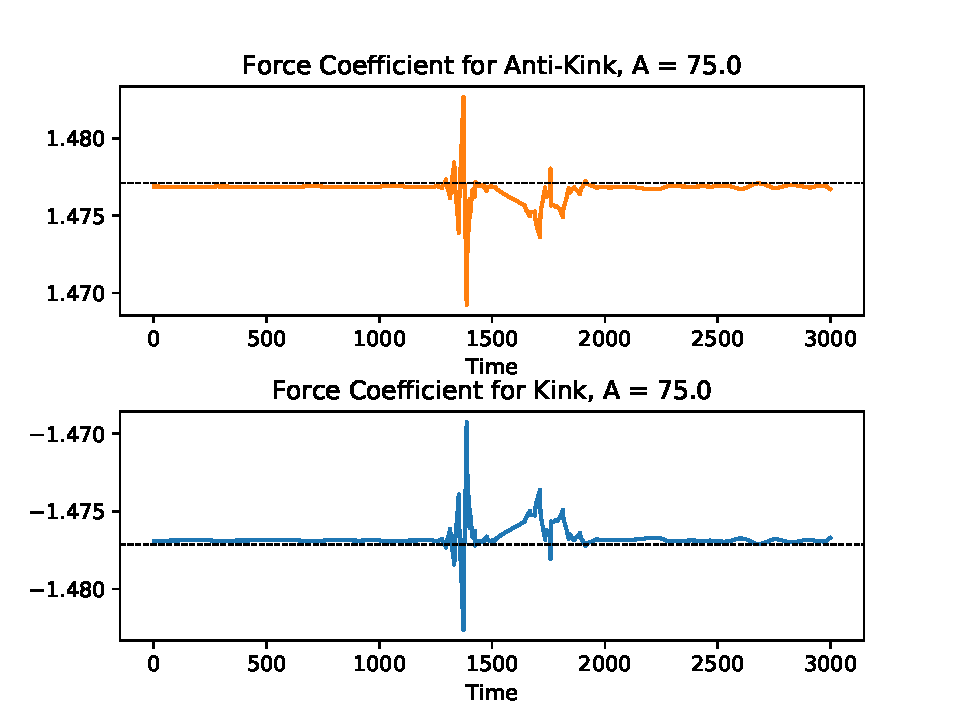
\includegraphics[width=0.3\textwidth]{force25}
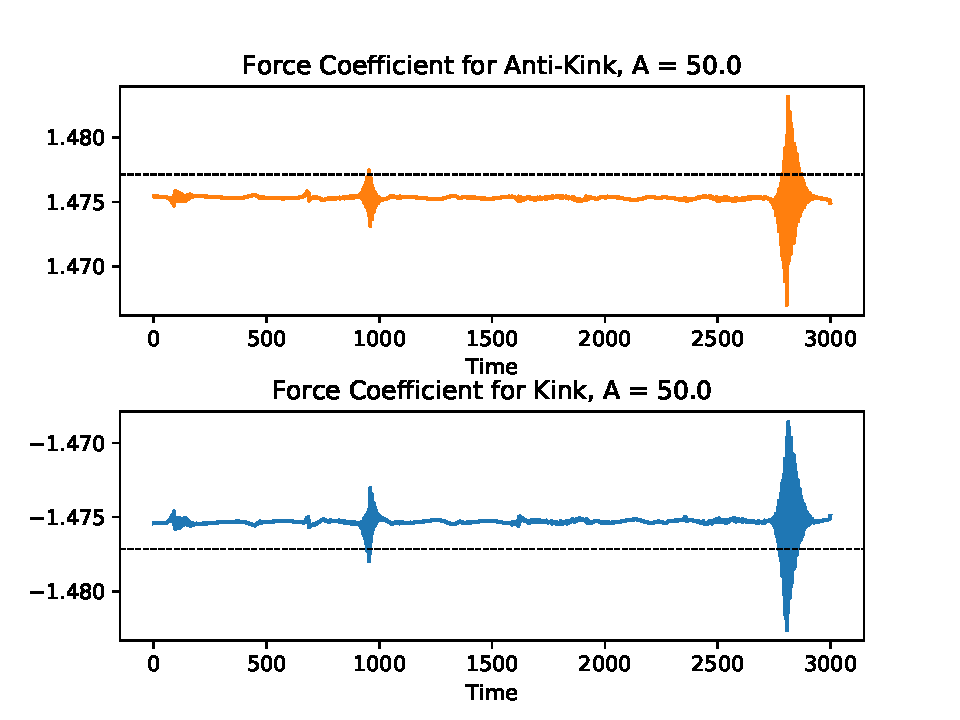
\includegraphics[width=0.3\textwidth]{force50}
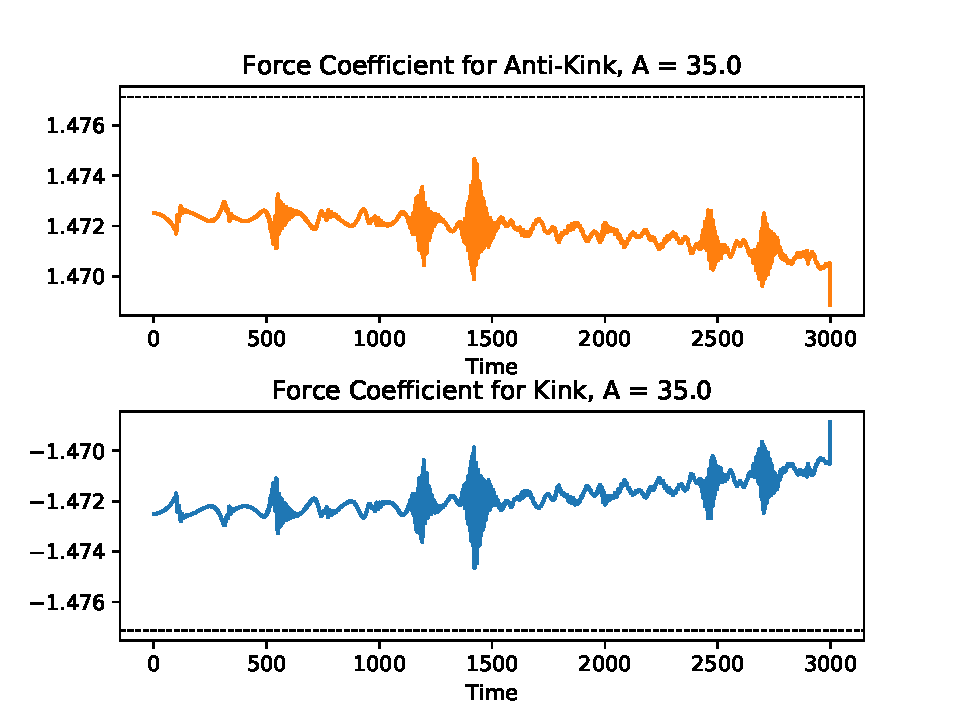
\includegraphics[width=0.3\textwidth]{force65}
\captionof{figure}{Plots of force coefficients against time for starting fields with $A=$ 75, 50 and 35. The value predicted in \textsection \ref{kink-kink-analytic} is marked with a dashed line.} \label{force_graphs}
\end{figure}

\subsection{Numerical Model for an Accelerating Kink}
We now take a different approach to numerically finding the strength of the force acting between a kink and anti-kink, focussing on carefully approximating the profile of an accelerating kink. Our starting point is eqn.~\ref{acc_kink}:
 \begin{equation}
 \chi'' - a\chi' - \frac{\drv V }{\drv \chi}=0.
 \end{equation}
 Note that in deriving this differential equation, the only approximation we took was to assume that $\dot{A}$ can be ignored, thus it is exact for finding the force acting on a static kink, before it has started to move under acceleration.\par
   \begin{wrapfigure}{r}{0.5\textwidth}
 \vspace{-10pt}
\centering
 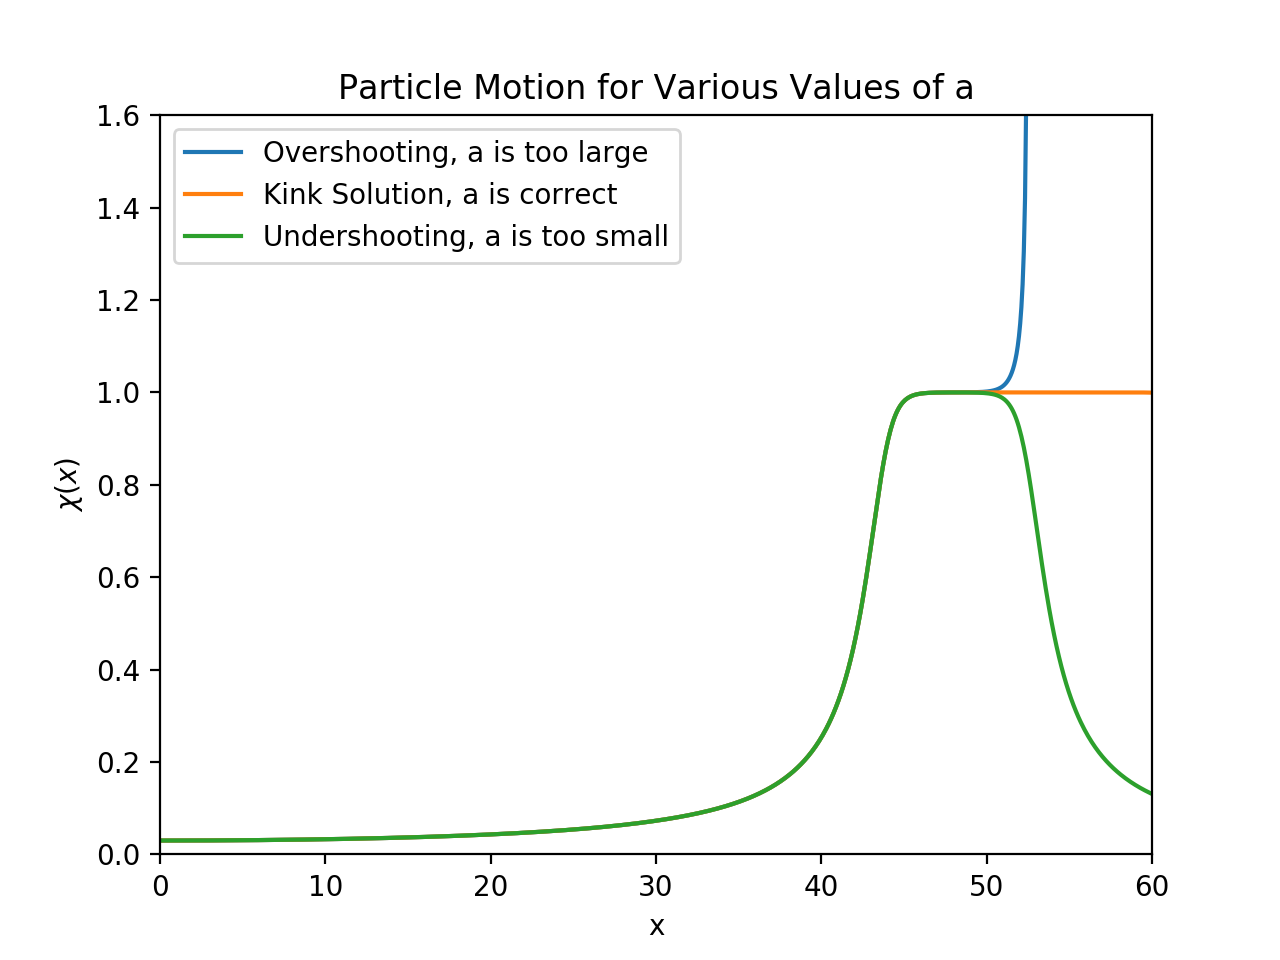
\includegraphics[width=0.5\textwidth]{over_under.png}
 \captionof{figure}{Plot of the particle's motion for three different values of $a$, with $\chi_0 = 0.003$. The correct value of $a$ is  $a_\textup{c} =  2.9763... \times 10^{-6}$ , where the overshooting value was $a_\textup{c} +\delta$ and the undershooting value was $a_\textup{c} -\delta$, for $\delta = 1\times 10^{-6}$} \label{over_under}
\end{wrapfigure} 
 We examine the differential equation through the lens of the mechanical interpretation, viewing it as describing a particle that starts at a position $\chi(0)$ and moves under negative drag term $-a$ in the potential $- \frac{\drv V }{\drv \chi}$. As explained in \textsection~\ref{kink-kink-analytic}, for every value of $\chi(0)$ there is a unique corresponding value of $a$ such that the motion of the particle will correspond to a valid kink solution. If a is too large, the particle will gain too much energy as it moves through the potential, overshooting the maximum and `falling off' the other side, accelerating towards $\chi \rightarrow +\infty$. If $a$ is too small, the particle will not gain enough energy as it moves through the potential, this means it won't make it up to the maximum of the potential at  $\chi=1$ and will turn back on itself, moving back towards negative $\chi$.\par
 This differential equation is easily solved, again using python's inbuilt ODE solver, \texttt{odeint}. We start with a choice of initial values, $\chi(0)$, $\chi'(0) = 0$ and $a$, and solve it for $\chi(x)$ for $x$ discretised over an array of length 2048.\par
To determine the correct value of $a$, given $\chi(0)$, we first decide on an upper and lower bound for $a$, $a_\textup{max}$ and $a_\textup{min}$, where we are certain that the particle moving under $\chi(0)$ with $a_\textup{max}$ will overshoot and a particle moving under $a_\textup{min}$ will undershoot. Now we determine the motion of the particle moving under $a_\textup{avg} = \frac{1}{2} \left ( a_\textup{max} + a_\textup{min} \right )$. If the motion under $a_\textup{avg}$ overshoots we know that the correct value of $a$ is somewhere between $a_\textup{min}$ and $a_\textup{avg}$, similarly if it undershoots we know that the correct value is between $a_\textup{avg}$ and $a_\textup{max}$. Thus we set a new pair of bounds $a_\textup{min, new}$ and $a_\textup{max, new}$ and repeat the process. Every time we iterate this step we are halving the size of the window that the correct value of $a$ is in, so we converge very quickly to the correct value. Figure \ref{over_under} shows the motion of the particle for three values of $a$, one with an overshoot, one that is correct and one that causes it to undershoot.\par
Once we have determined the correct value of $a$, we automatically get an expression for the shape of an accelerating kink for our chosen $\chi(0)$ as the solution of our differential equation. Now the only thing left to do is to find the position of the center of the kink, A, by looking for the point in space where the kink crosses $\chi(A) = \phi_\textup{kink}(x=0) \approx 0.8335$. The force acting on the kink is given by eqn.~\ref{force}, $F = -V[\chi(0)]$. Thus we have arrived at a set of values for the force acting on the kink as a function of the kink separation. The results of this are plotted in fig.~\ref{force_distance_trick}, plotted against the predicted relationship derived in \textsection~\ref{kink-kink-analytic}, $F = 1.4771A^{-4}$. As can clearly be seen, the results are extremely close, with some deviation from the predicted values as the kinks get closer together, which is expected since our analytic methods relied on the kinks being well separated.
\begin{figure}
\centering
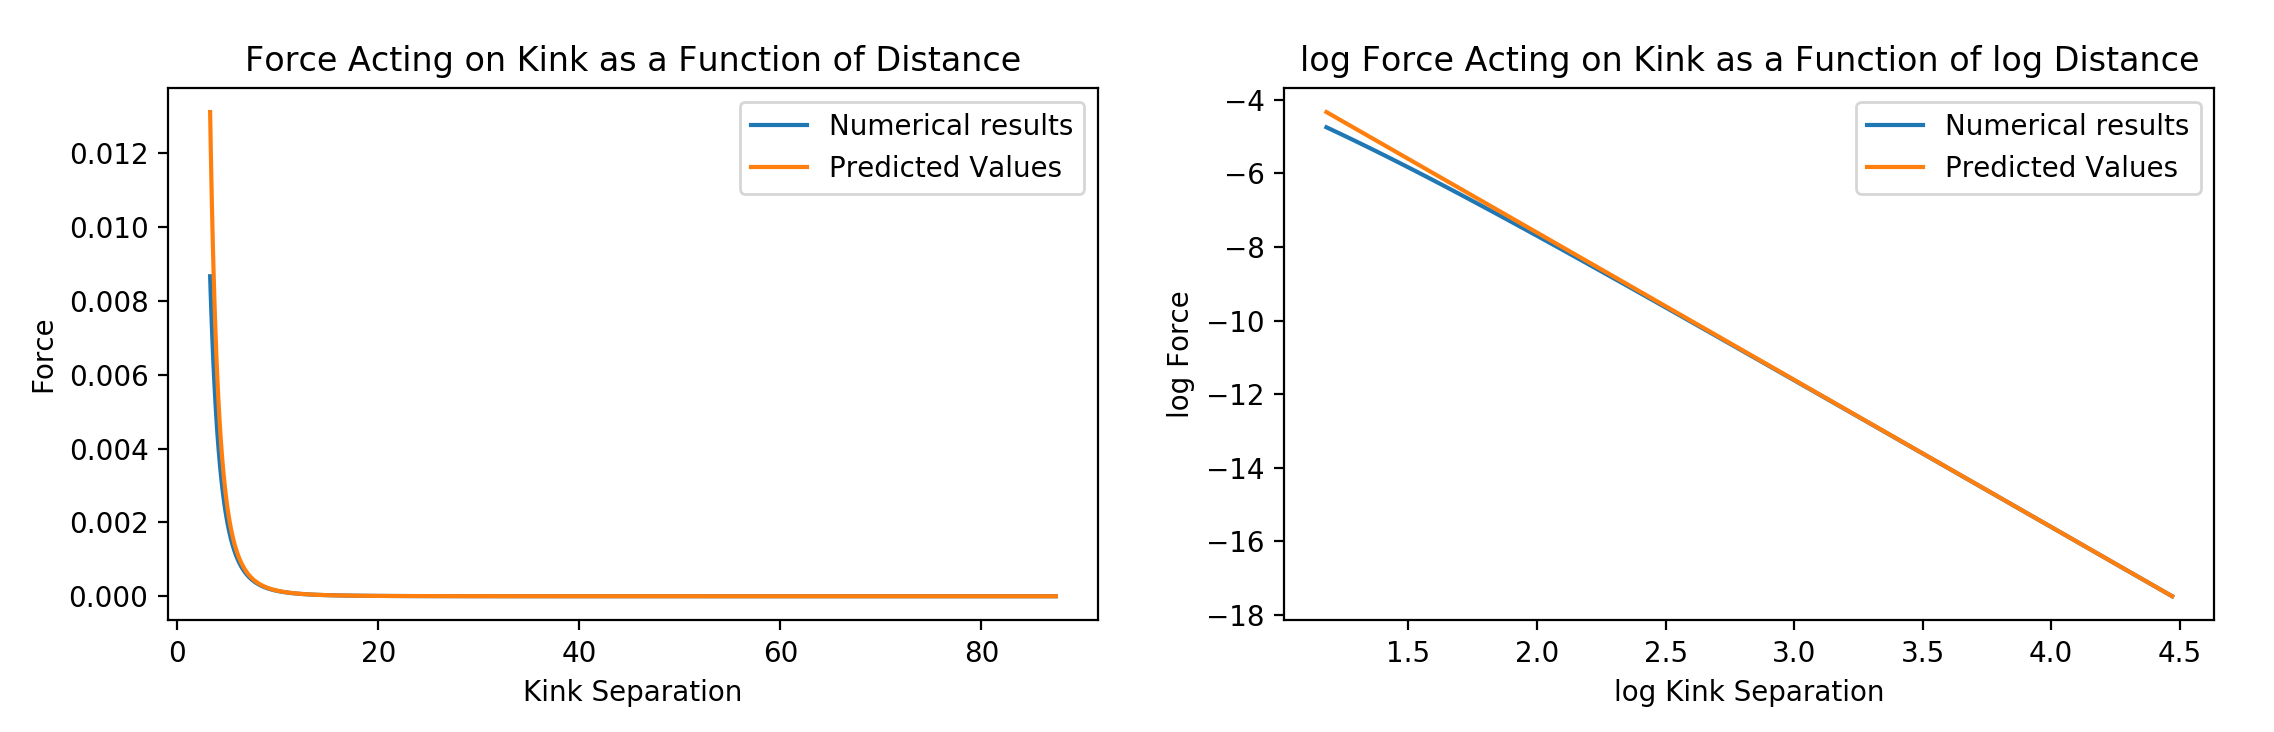
\includegraphics[width=0.9\textwidth]{force_distance_trick.png}
\captionof{figure}{The left plot shows the relationship between the kink separation and the force acting between the kinks. On the right is the same data plotted on a log-log scale. The predicted results have a polynomial relationship and so appear here as a straight line. It can be seen that the numerically calculated force is slightly weaker than expected when the kinks are close, but extremely close to prediction once the kinks are well separated.} \label{force_distance_trick}
\end{figure}

 \section{Kink-Radiation Interactions}\label{kink_radiation}
 Thus far, we have stressed that, in all calculations, the most important consideration is to ensure that the field is initialised into the correct state before analysing its dynamics. A particularly extreme example of this may be seen in \cite{belendryasova} where the interactions between kinks and anti-kinks were simulated using the sum ansatz described in \textsection \ref{kink_kink_comp}. Not only was the strength of the inter-kink force wrong here but the sign as well, predicting that kinks and anti-kinks repelled, clearly in contradiction to the results obtained in all of our calculations. This phenomenon is corroborated in \cite{christov-num}, where a number of initial conditions are explored, and repulsive dynamics are observed in the vast majority of imperfectly initialised states. Here we aim to understand the reasons for this dramatic sensitivity to initial conditions. In the vast majority of cases, imperfect initialisation starts the field with an excess of energy that is emitted as radiation. This radiation then interacts with the kinks, affecting their motion. Thus in this section we aim to understand the nature of interactions between these long-range kinks and radiation. We start with a number of numerical simulations, and then look at modelling these effects analytically in \textsection \ref{rad-anal}. \par
 Before diving into the simulations, we derive a few elementary facts about radiation in our theory. We start with the equations of motion for the field
 \begin{equation}
 \ddot{\phi} - \phi'' + V'(\phi) = 0
 \end{equation}
and expand the solution around one of the vacua $\phi = \phi_0 + \xi$, with $\xi$ small. Thus, the potential may be expanded about $\phi = \phi_0$ according to
\begin{equation}
\ddot{\xi} -\xi'' + \xi V''(\phi_0) = 0
\end{equation}
since $V'(\phi_0) = 0$. Thus, for radiation with small amplitude, the EOM is the Klein-Gordon equation, where the `mass term' ($m^2 = V''(\phi_0)$) depends on the choice of vacuum. In $\phi^8$ theory, $V'' = 6\phi^2 -30\phi^4 + 28\phi^6$. Around $\phi_0 = 0$, $m^2 = 0$ so the field is massless. Around $\phi_0 = \pm1$, $m^2 = 4$, the field is massive. We now find plane-wave solutions to the Klein-Gordon equation ($\ddot{\xi} - \xi'' + m^2\xi = 0$) using the ansatz
\begin{equation}
\xi(x,t) = \mathcal{A}e^{i(kx-\omega t)}.
\end{equation}
Plugging this into the KG equation yields the dispersion relation
\begin{equation}
\omega^2 = k^2 + m^2.
\end{equation}
Thus on the massless side $\omega = |k|$ and on the massive side $\omega = \sqrt{k^2 + 4}$. In this work we will be looking at wave-packet solutions of the Klein-Gordon equations. These are found by integrating a continuous spectrum of plane-wave solutions with gaussian distribution, according to 
\begin{figure}
\centering
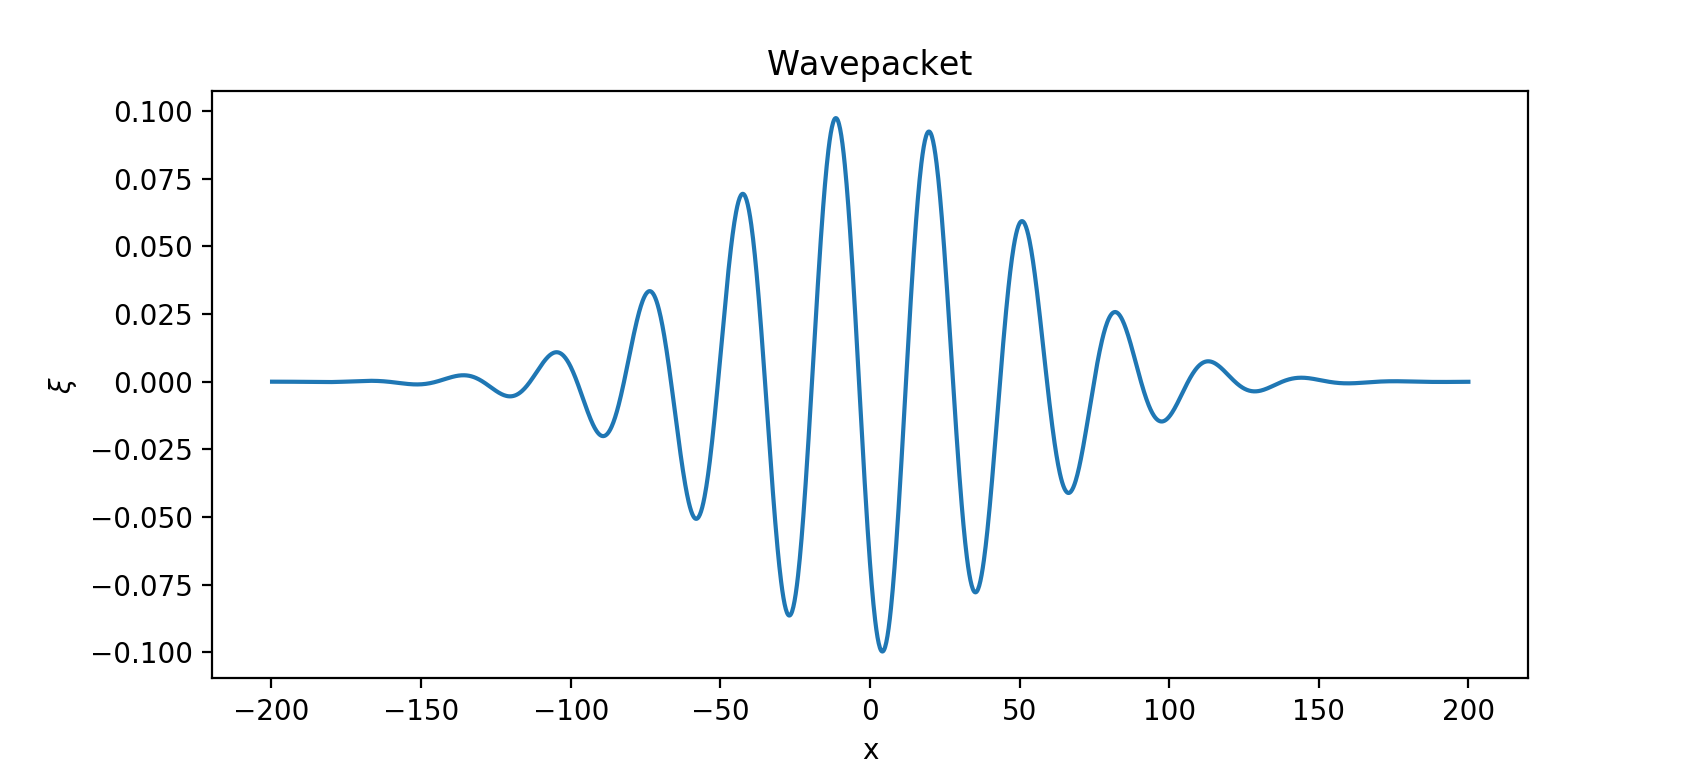
\includegraphics[width=0.5\textwidth]{wavepacket.png}
\captionof{figure}{An example wave-packet with $k_0$ = 0.2, $\Delta_x = 50$ ($\Delta_k = 0.0001$) and $\tilde{\mathcal{A}} = 0.1$} \label{wavepacket}
\end{figure}
\begin{equation}
\xi (x,t) =\mathcal{A} \int \frac{\drv k}{2\pi} \exp\left[{i(kx-\omega t)} - \frac{(k-k_0)^2}{4\Delta_k^2} \right]
\end{equation}
where $k_0$ is the central wave-vector of the gaussian distribution and $\Delta_k$ is the standard deviation. To simplify the calculation we make the approximation that $\Delta_k$ is small, so the gaussian is tightly bunched around the central value and the expression only has support for $k$ close to $k_0$, thus we may approximate $\omega \simeq \omega_0 = \sqrt{k_0^2 +m^2}$. The expression becomes
\begin{equation} \label{wave_eqn}
\xi =\mathcal{A}e^{-i\omega_0 t} \int \frac{\drv k}{2\pi} \exp\left[{ikx} - \frac{(k-k_0)^2}{4\Delta_k^2} \right]
\end{equation}
which can be solved using the standard integral
\begin{equation}
\int_{-\infty}^{\infty} \drv k\exp \left ( -\alpha k^2 + \beta k \right ) = \sqrt{\frac{\pi}{\alpha}}\exp\left( \frac{\beta^2}{4\alpha}\right ) 
\end{equation}
to give
\begin{equation}
\xi =\tilde{\mathcal{A}}e^{i(k_0 x-\omega_0 t)} e^{-\frac{x^2}{4\Delta_x^2}}
\end{equation}
with $\tilde{\mathcal{A}} = \frac{\mathcal{A}}{\sqrt{\pi}}\Delta_k $ and $\Delta_x^2 = \frac{1}{4\Delta_k^2}$. Note that a small $\Delta_k$ implies that $\Delta_x$ is large, the wave-packet must have large spatial extent. Figure \ref{wavepacket} shows an example wave-packet.

 \subsection{Numerical Work} \label{kink_rad_numerics}
We simulate the equations of motion in the same manner as in \textsection \ref{kink_kink_comp}, by splitting the PDE into a large number of coupled ODEs and approximating the spatial derivatives using spectral methods. In this case, however, we are modelling the interactions between a single kink and radiation. To impose periodic boundary conditions onto a field with a single kink only we have to resort to some trickery. We split the field into a static background kink term and a radiation term.
\begin{equation}
\phi(x,t) = \phi_{\textup{kink}}(x) + \xi(x,t)
\end{equation}
where $\phi_{\textup{kink}}(x)$ is the static solution for a field containing a single kink with $A=0$, determined by eqn.~\ref{long_kink_eq}. $\xi(x,t)$ is a dynamical term that contains the radiation interacting with the kink. The equations of motion may then be re-expressed as
\begin{equation}
\ddot{\xi} - \xi'' - \phi''_\textup{kink} + V' \left( \phi_\textup{kink} + \xi \right)= 0.
\end{equation}
Note that all we have done is subtract the static solution for a kink. The kink is still free to move as the system evolves. Any displacement of the kink will also be contained in $\xi(x,t)$, and the final solution is obtained by adding $ \phi_{\textup{kink}}(x)$ and $\xi(x,t)$. The main purpose of subtracting away the static kink solution is to enforce periodic boundary conditions, allowing us to use spectral methods in our numerics. Figure \ref{kink-rad-init} shows a profile for a field containing a kink and radiation, and the same field with the kink subtracted away. We have used wave-packets rather than plane waves, again in order to preserve periodic boundary conditions.\par
\begin{figure}
\centering
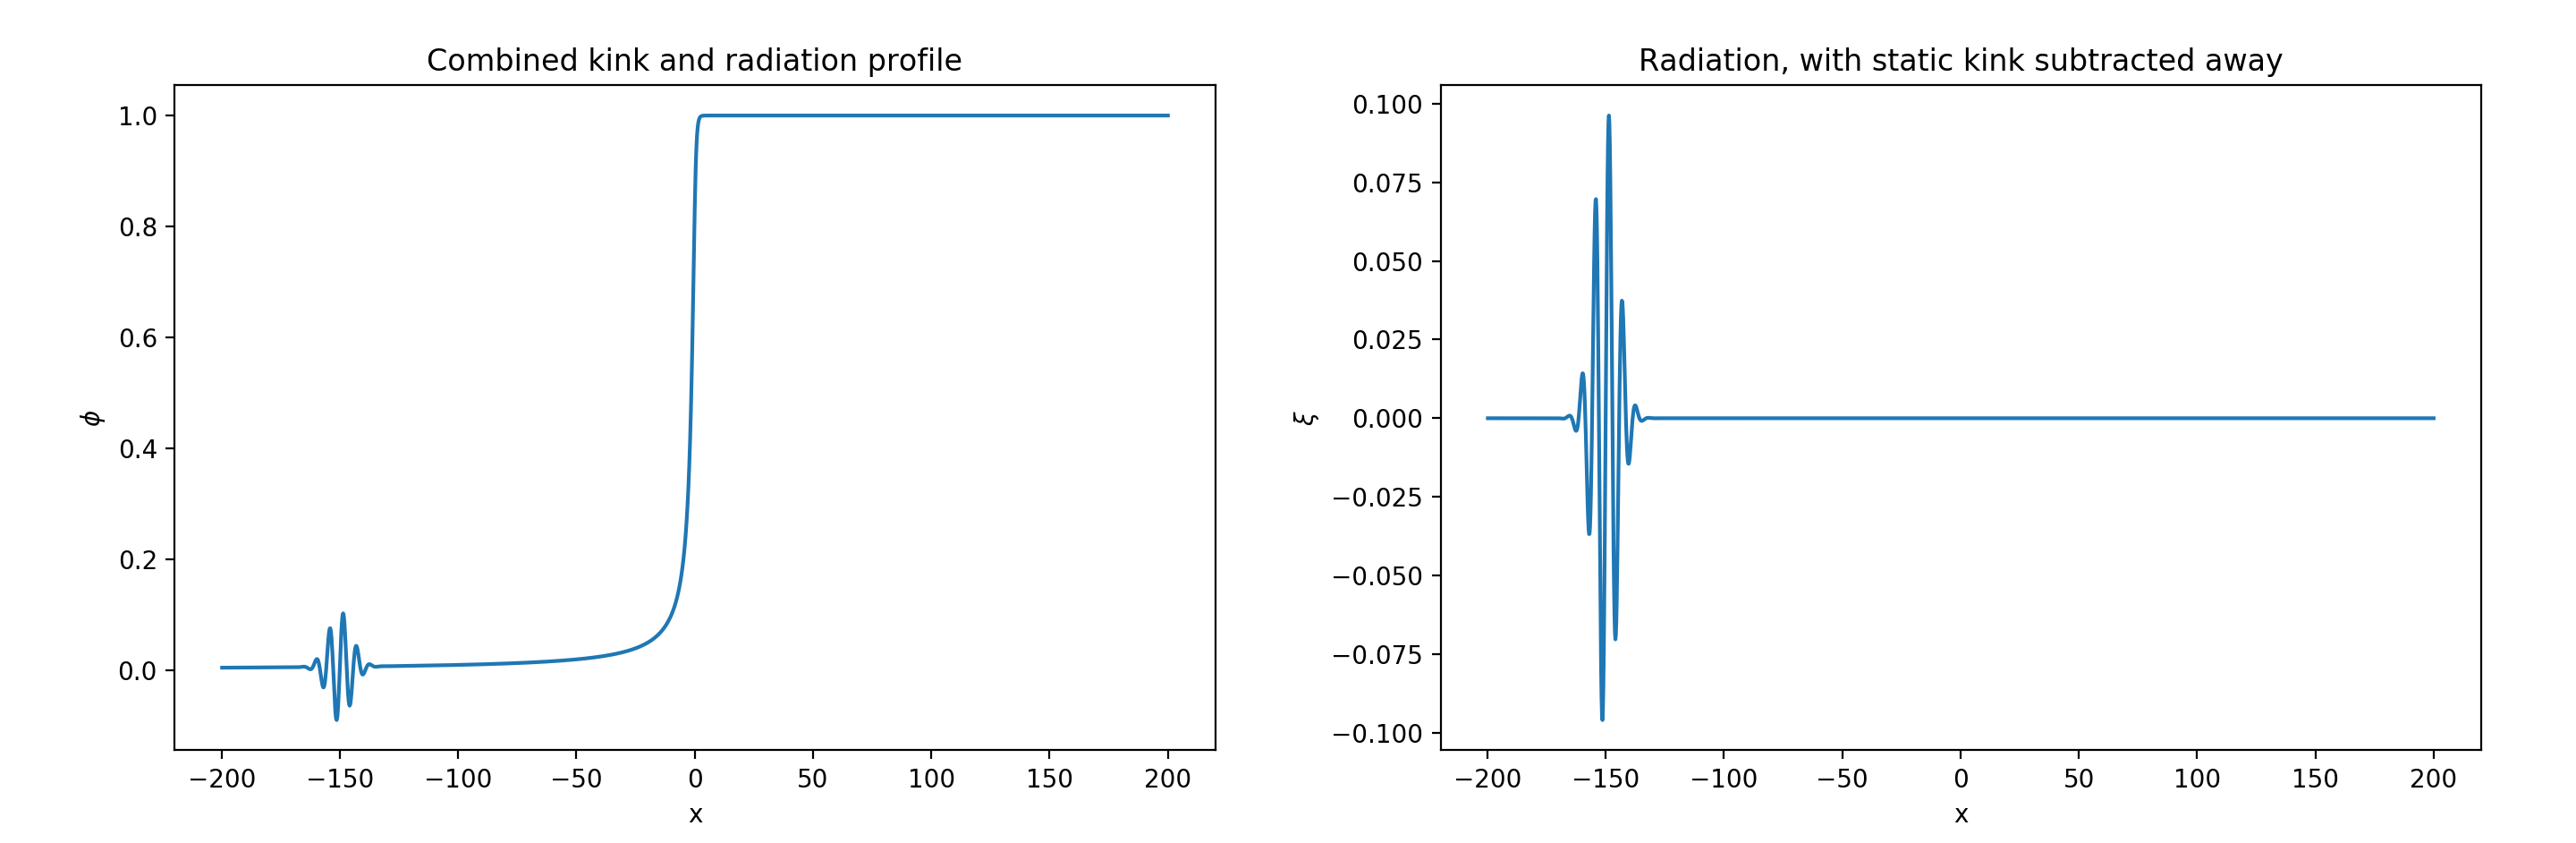
\includegraphics[width=0.8\textwidth]{kink_rad_init}
\captionof{figure}{Profile containing a kink and pulse of radiation at $X=50$, on the right the $\xi$ field is shown, with the kink subtracted away, allowing for periodic boundary conditions.} \label{kink-rad-init}
\end{figure}
We ran two sets of simulations, one with radiation approaching a kink from the left, starting in the massless regime with $\omega = |k|$. The second set starts with radiation on the massive side, with $\omega = \sqrt{k^2 + 4}$. In all cases the wave-packet had the same spatial extent, with $\Delta_x = 5$, giving $\Delta_k = 0.01$. Scattering was tested for wave-packets with values of $k_0$ ranging from 1.5 to 3, stepping up in increments of 0.125. Thus, in all cases $\Delta_k$ contributes a correction to $k$ of less than 1\% and so the assumption made in eqn.~\ref{wave_eqn} is valid. Equation \ref{momentum} was used to numerically calculate the total momentum of the wave-packet and the amplitude, $\mathcal{A}$, was set to ensure that the total momentum of every wave-packet was 0.01.\par
\begin{figure}
\centering
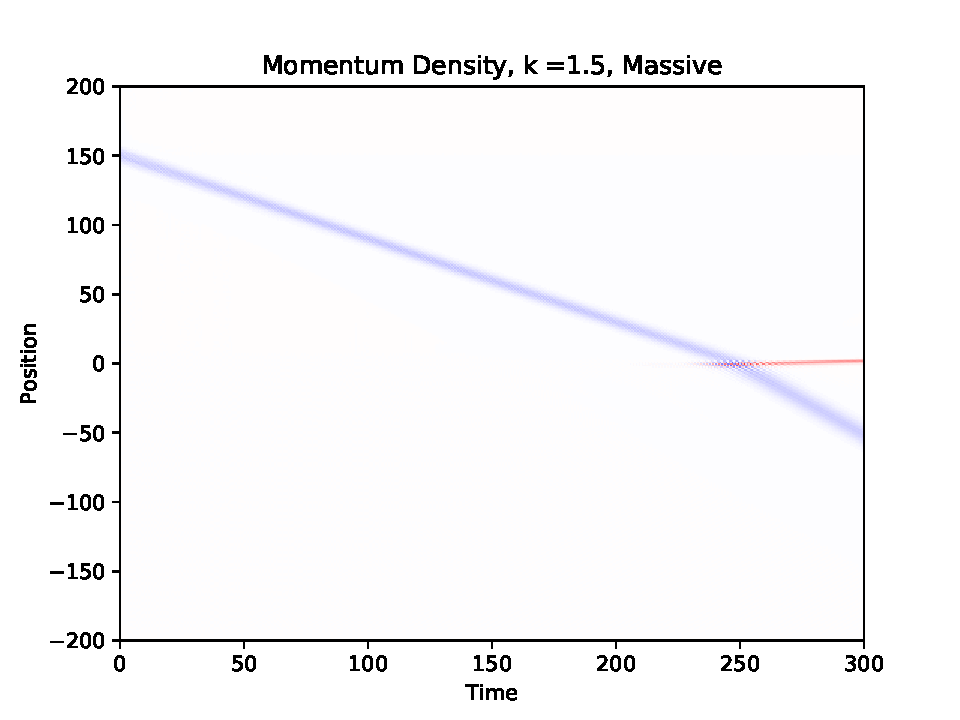
\includegraphics[width=0.3\textwidth]{MomentumDensityk15Massive.pdf}
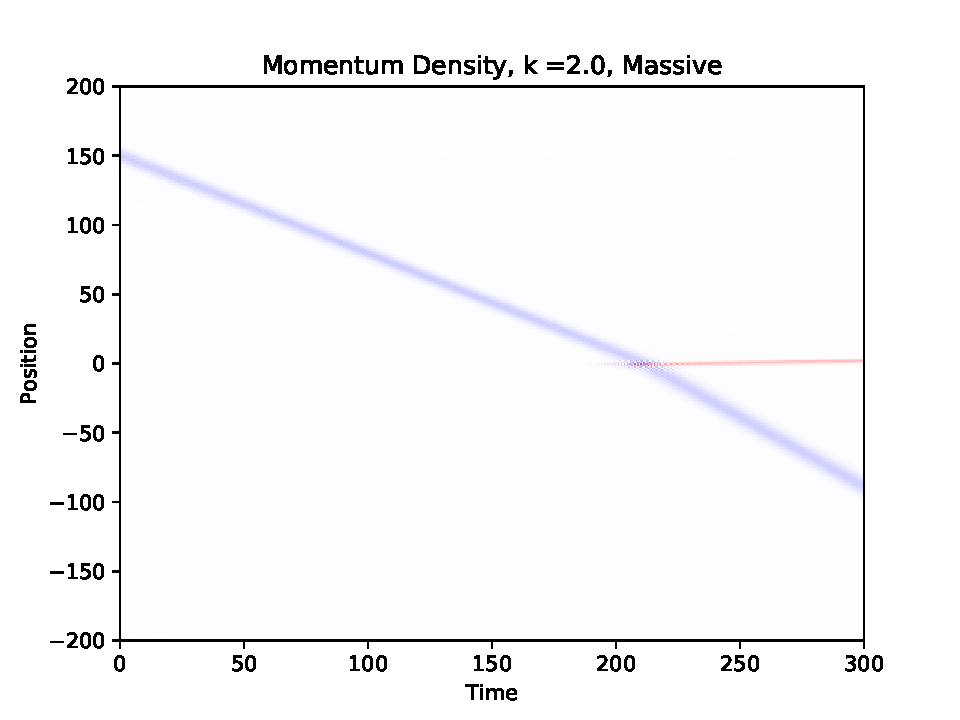
\includegraphics[width=0.3\textwidth]{MomentumDensityk20Massive.pdf}
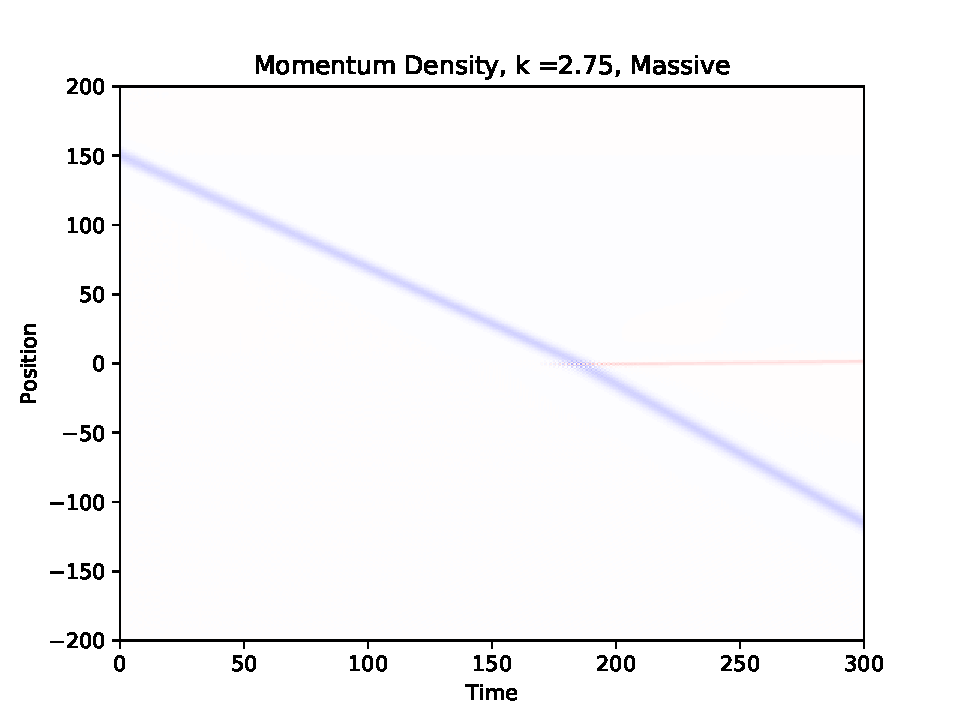
\includegraphics[width=0.3\textwidth]{MomentumDensityk275Massive.pdf}
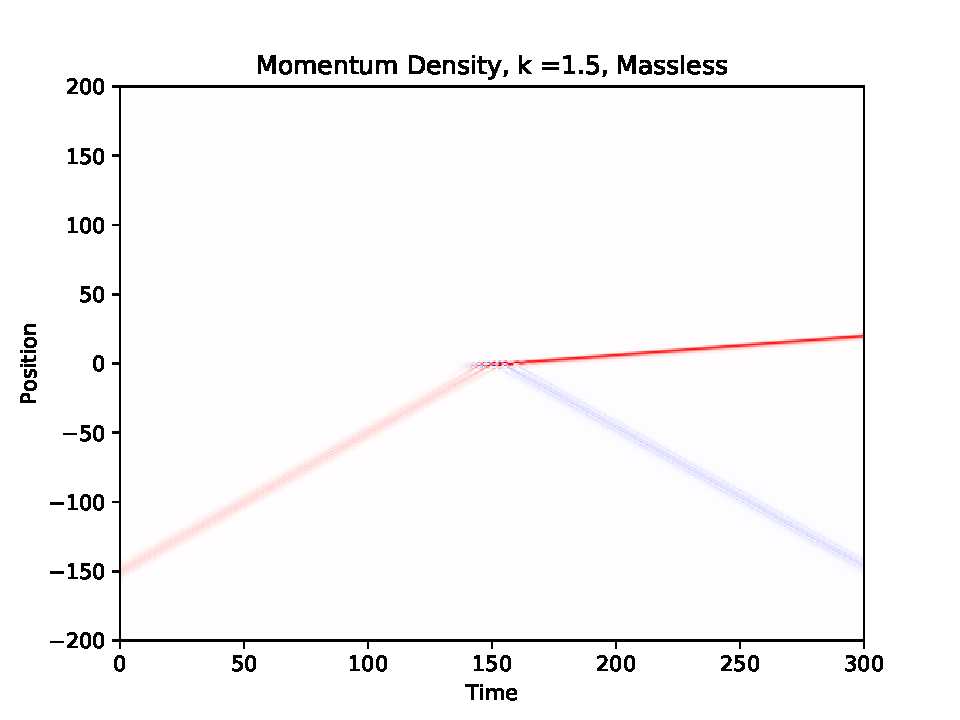
\includegraphics[width=0.3\textwidth]{MomentumDensityk15Massless.pdf}
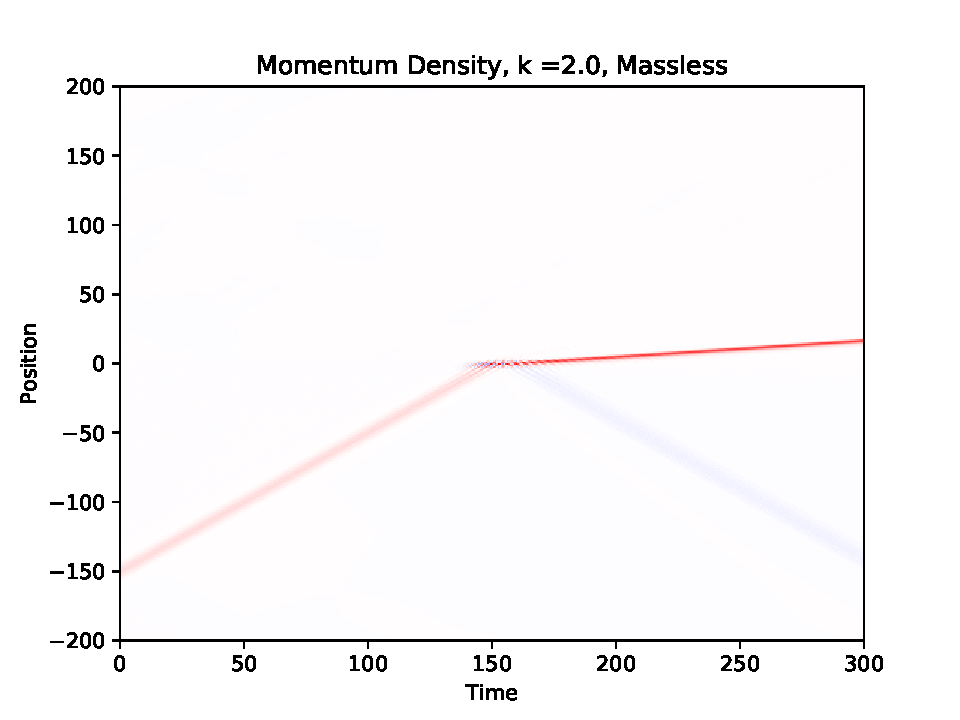
\includegraphics[width=0.3\textwidth]{MomentumDensityk20Massless.pdf}
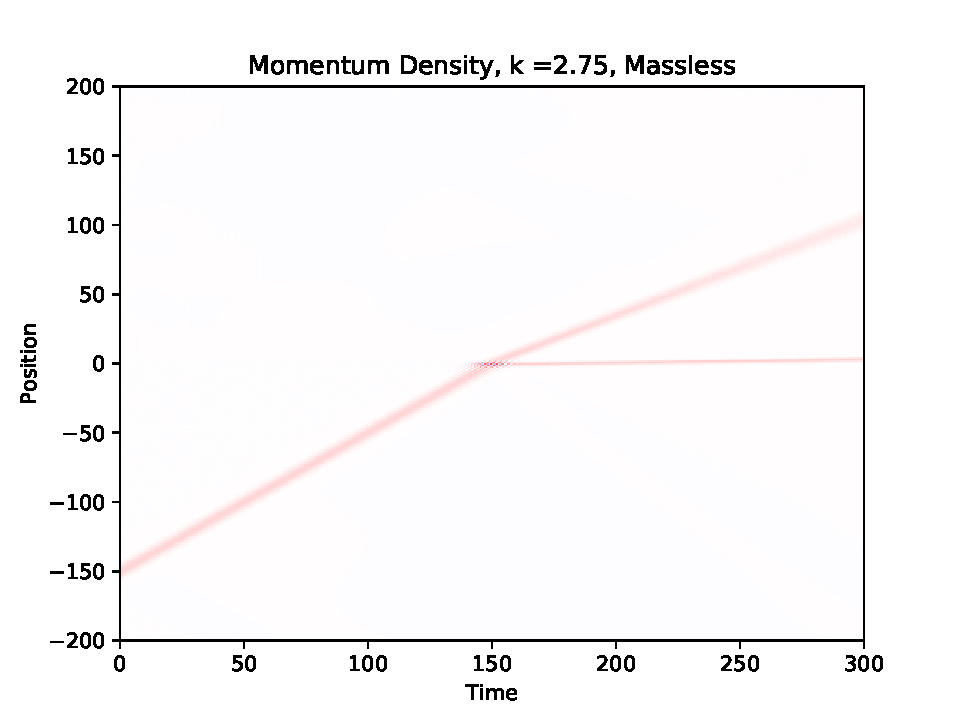
\includegraphics[width=0.3\textwidth]{MomentumDensityk275Massless.pdf}
\captionof{figure}{Plots of the momentum density of the field as a function of space and time coordinates for a set of wave-packets with central wavenumber $k = 1.5$, 2.0 and 2.75. In this image, blue marks regions of negative momentum and red marks regions of positive momentum.} \label{radiation_results}
\end{figure}
In all simulations the kink is initially centred at $x=0$ and the wave-packet starts at position $x=\pm150$, with the sign determining whether it starts on the massive or massless side. In order to display the results clearly, the momentum density is calculated and plotted, clearly depicting the motion of the wave-packet. The kink is initially static at $x=0$, so has no momentum and does not show up in the plot. After collision with radiation, however, it can be clearly seen. These results are shown in fig.~\ref{radiation_results}. A comprehensive set of results, complete with animations, may be found at https://github.com/dpreuo/Kinks-and-radiation\par
There are two effects taking place here worth discussing. The first and most striking is that radiation coming from the massless side of the kink is reflected for $k < 2$ and transmitted for $k>2$. At $k = 2$ it is majority reflected, but a small amount is transmitted. This effect is most clearly seen in animations of the collision, since not enough radiation is transmitted to show up clearly in the momentum plots. The second important effect taking place here is that regardless of the wavenumber or direction of incoming radiation, the kink always exits the collision with positive momentum. 

 \subsection{Analytic Models} \label{rad-anal}
 We propose two models for understanding the behaviour seen in \textsection \ref{kink_rad_numerics}. The first looks at perturbatively modelling the potential felt by radiation as it crosses the kink. By calculating the coefficients of reflection and transmission it is possible to infer the strength and direction of the force acting on the kink. Secondly we will look at the effect of background radiation on the potential by averaging out a small background term to obtain an effective potential acting on the kink.
 \subsubsection{Perturbation Theory} \label{pert_theory}
Start with the equations of motion for a static background containing a kink at $x=0$, $\phi_\textup{kink}(x)$ and a small radiation term $\xi(x,t)$
\begin{equation}\label{EOM_rad}
\ddot{\xi} - \xi'' - \phi''_\textup{kink} + V' \left( \phi_\textup{kink} + \xi \right)= 0.
\end{equation}
We Taylor expand the potential to first order, treating $\xi$ as a small perturbation:
 \begin{equation}
 V' \left( \phi_\textup{kink} + \xi \right) = V' \left( \phi_\textup{kink} \right ) + \xi V'' \left( \phi_\textup{kink}\right) + \mathcal{O}\left(\xi^2 \right ).
 \end{equation}
 Substituting this into eqn.~\ref{EOM_rad} and using the fact that $\phi_\textup{kink}$ satisfies the static equations of motion for the field, $\phi_\textup{kink}'' - V'(\phi_\textup{kink}) = 0$ gives us
 \begin{equation}
\ddot{\xi} - \xi'' + \xi V'' \left( \phi_\textup{kink}\right)= 0.
\end{equation}
This equation looks similar to the Klein-Gordon equation with an effective mass term that has nontrivial spatial dependence, $m^2(x) = V''\left[\phi_\textup{kink}(x)\right]$. Figure \ref{mass_term} shows a plot of the effective mass as a function of spatial coordinate.\par
We can now look at analysing the reflection and transmission of plane waves crossing the kink. The kink's profile is only implicitly defined by eqn.~\ref{long_kink_eq}, so the profile of $m^2(\phi_{\textup{kink}})$ also lacks an explicit expression and must be determined numerically. In order to calculate the wave's behaviour analytically, we approximate this as a step function
\begin{equation}
m^2 (x) =\left\{\begin{matrix}
0, \; x<0\\ 
4, \; x>0
\end{matrix}\right. .
\end{equation}
\begin{wrapfigure}{r}{0.45\textwidth}
\centering
 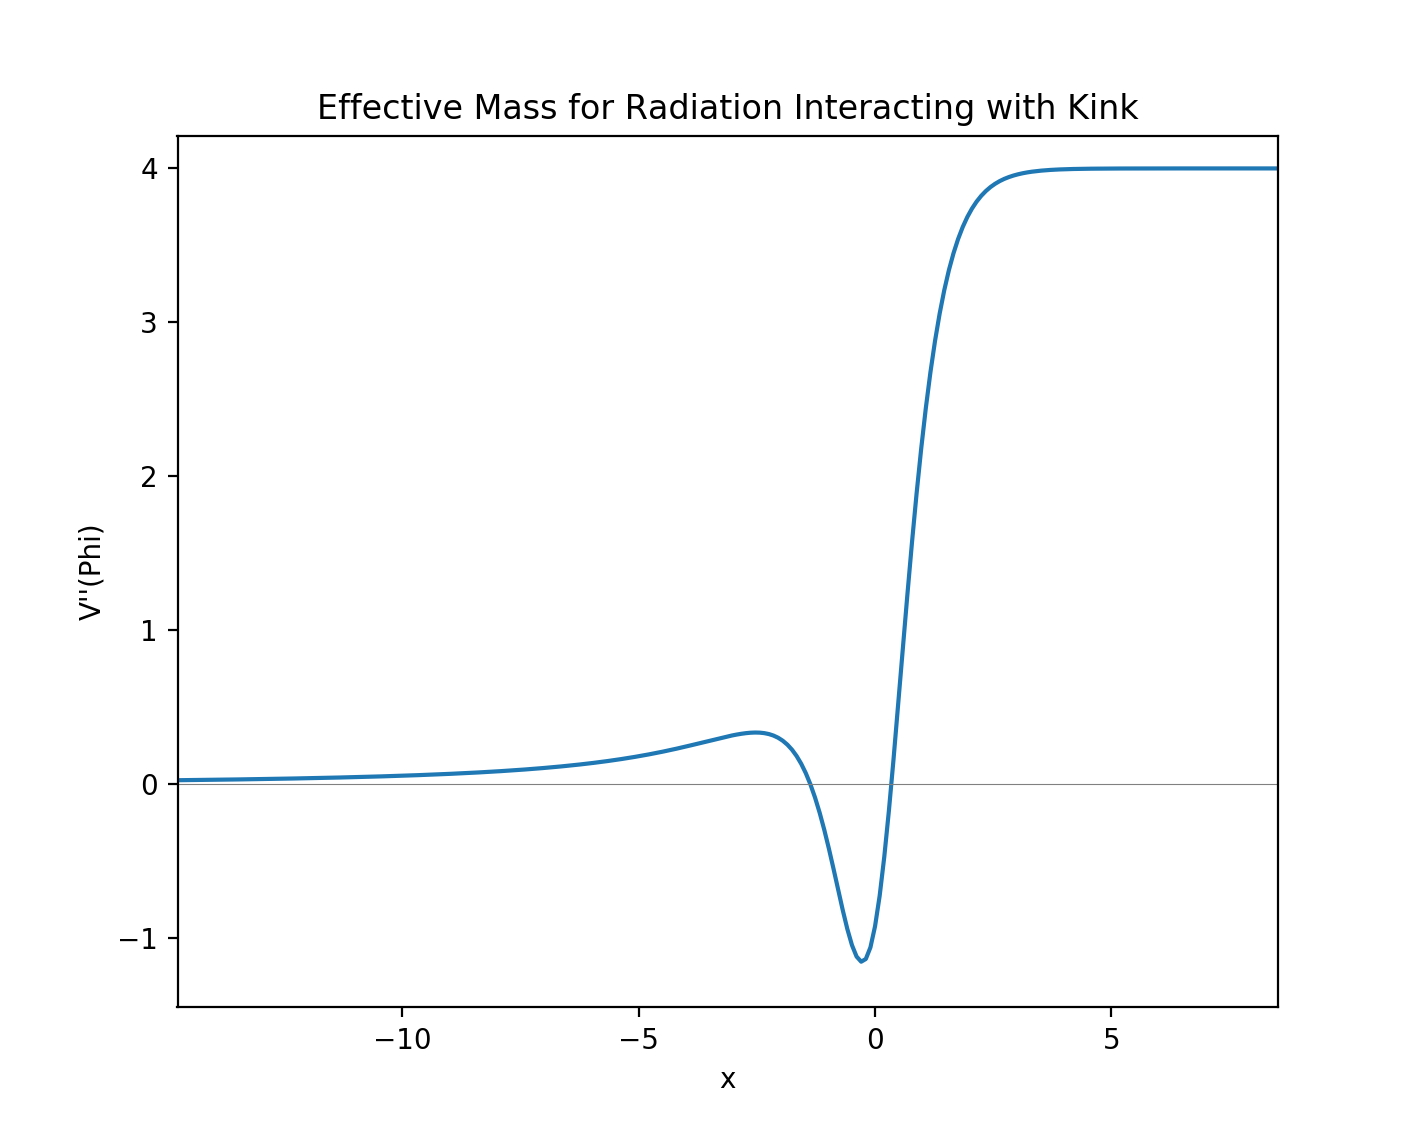
\includegraphics[width=0.45\textwidth]{mass_term.png}
 \captionof{figure}{Effective mass felt by radiation} \label{mass_term}
\end{wrapfigure}
On the far left and far right of the the kink, the equation reduces to the regular Klein-Gordon equation with $m^2 = $ 0 or 4. The radiation in those limits may be described by the following expression.
\begin{equation}
\xi(x,t) = \mathcal{A}e^{i(kx-\omega t)}
\end{equation}
with $\omega = \sqrt{k^2 + m^2}$, as explained at the start of \textsection \ref{kink_radiation}. We expect that there will be reflection and transmission at the boundary ($x=0$), so we propose the following solutions for the field corresponding to a plane wave hitting the boundary, coming from $x<0$ with frequency $\omega$.
\begin{align}
\xi_\textup{left} &= e^{-i\omega (t-x)} + Re^{-i\omega (t+x)} + \textup{c.c.} \label{wave_left}\\
\xi_\textup{right} &= T e^{-i(\omega t-\sqrt{\omega^2 - 4}x)} + \textup{c.c.} \label{wave_right}
\end{align}
We now calculate the coefficients, $R$ and $T$, by enforcing continuity for the field and its first derivative at the boundary
\begin{align}
\xi_\textup{left}(t,x=0) &= \xi_\textup{right}(t,x=0) \label{cont1}\\
\xi'_\textup{left}(t,x=0) &= \xi'_\textup{right}(t,x=0). \label{cont2}
\end{align}
From these two requirements we derive the relations
\begin{align}
1+R = T\\
1-R = \sqrt{1-\frac{4}{\omega^2}}T.
\end{align}
Setting $\alpha = \sqrt{1-\frac{4}{\omega^2}}$ we arrive at
\begin{align} \label{RT}
R = \frac{1-\alpha}{1+\alpha}, \;\; T = \frac{2}{1+\alpha}.
\end{align}
The first effect worth mentioning is that for $\omega < 2$ the term $\sqrt{\omega^2 - 4}$ is imaginary and so the wave on the right hand side of the boundary has the form $ \xi_\textup{right} \sim e^{-\sqrt{\omega^2 - 4}x}$. No wave is transmitted. Furthermore, $\alpha$ is imaginary and the magnitude of $R$ is 1, meaning the wave is fully reflected. This explains the effects seen in fig.~\ref{radiation_results} where the kink completely reflected radiation coming from the massless side with $\omega < 2$. In the following derivation it is assumed that $\omega> 2$ and $\alpha$, $R$ and $T$ are real, we deal with $\omega< 2$ separately. Additionally, in the limit of large $\omega$, $\alpha \rightarrow 1$ and $R\rightarrow0$ and $T \rightarrow 1$. No radiation is reflected and the kink becomes transparent.\par
The momentum density of a wave is given by $\mathcal{P} = -\dot{\xi}\xi'$. Thus, from the real parts of eqn.~\ref{wave_left} and \ref{wave_right} the momentum density of the wave on the left and right side of the kink is given by
\begin{align}
\mathcal{P}_\textup{left} &= \omega^2 \sin^2\left[\omega(t-x)\right] - R^2 \omega^2 \sin^2\left[\omega(t+x)\right]\\
\mathcal{P}_\textup{right} &= T^2 \omega \sqrt{\omega^2 - 4} \sin^2\left( \omega t - \sqrt{\omega^2 - 4} x\right ).
\end{align}
Note that here we have ignored cross terms between the incident and reflected wave, since they average to 0 over a wavelength. Finally, averaging over a wave period gives
\begin{align}
 \left \langle \mathcal{P}_\textup{left} \right \rangle &= \frac{1}{2}\omega^2 \left ( 1 - R^2 \right) \\
 \left \langle \mathcal{P}_\textup{right} \right \rangle &= \frac{1}{2}T^2 \omega^2 \alpha.
\end{align}
The force on the boundary is given by the total flux of momentum coming into that point, given by
\begin{equation}
F = \sum_\textup{l,r} \mathcal{P} v_g
\end{equation}
where $v_g$ is the group velocity of the wave, given by
\begin{equation}
v_g = \frac{\partial \omega}{\partial k} = \frac{\partial }{\partial k} \sqrt{k^2+m^2} = \frac{k}{\sqrt{k^2+m^2}} = \frac{k}{\omega}.
\end{equation}
On the massless side, $m^2 = 0$ so $v_g = 1$ and the force acting on the kink is
\begin{equation}
F_\textup{left} = \frac{1}{2}\omega^2 \left ( 1 + R^2 \right).
\end{equation}
On the massive side, $m^2 = 4$ so $v_g = \frac{\sqrt{\omega^2 - 4}}{\omega} = \alpha$ and the force acting on the kink is
\begin{equation}
F_\textup{right} = -T^2 \omega^2 \alpha^2.
\end{equation}
The total force is
\begin{equation}
F = \frac{1}{2}\omega^2 \left ( 1 + R^2-T^2\alpha^2\right).
\end{equation}
Now, using eqn.~\ref{RT} to put in the explicit forms of $R$ and $T$ we arrive at
\begin{equation}
F = \omega^2 \frac{1-\alpha^2}{\left (1+\alpha \right ) ^2}.
\end{equation}
When $\omega<2$ the wave is fully reflected, with the magnitude of R being 1. The momentum densities of the incident and transmitted waves are both $\frac{1}{2}\omega^2$, with group velocity $v_g=1$ so the total force acting on the kink is 
\begin{equation}
F = \omega^2.
\end{equation}
A plot of the force as a function of frequency for waves approaching the kink from the massless side is shown in figure \ref{force_left}.\par
\begin{figure}
\centering
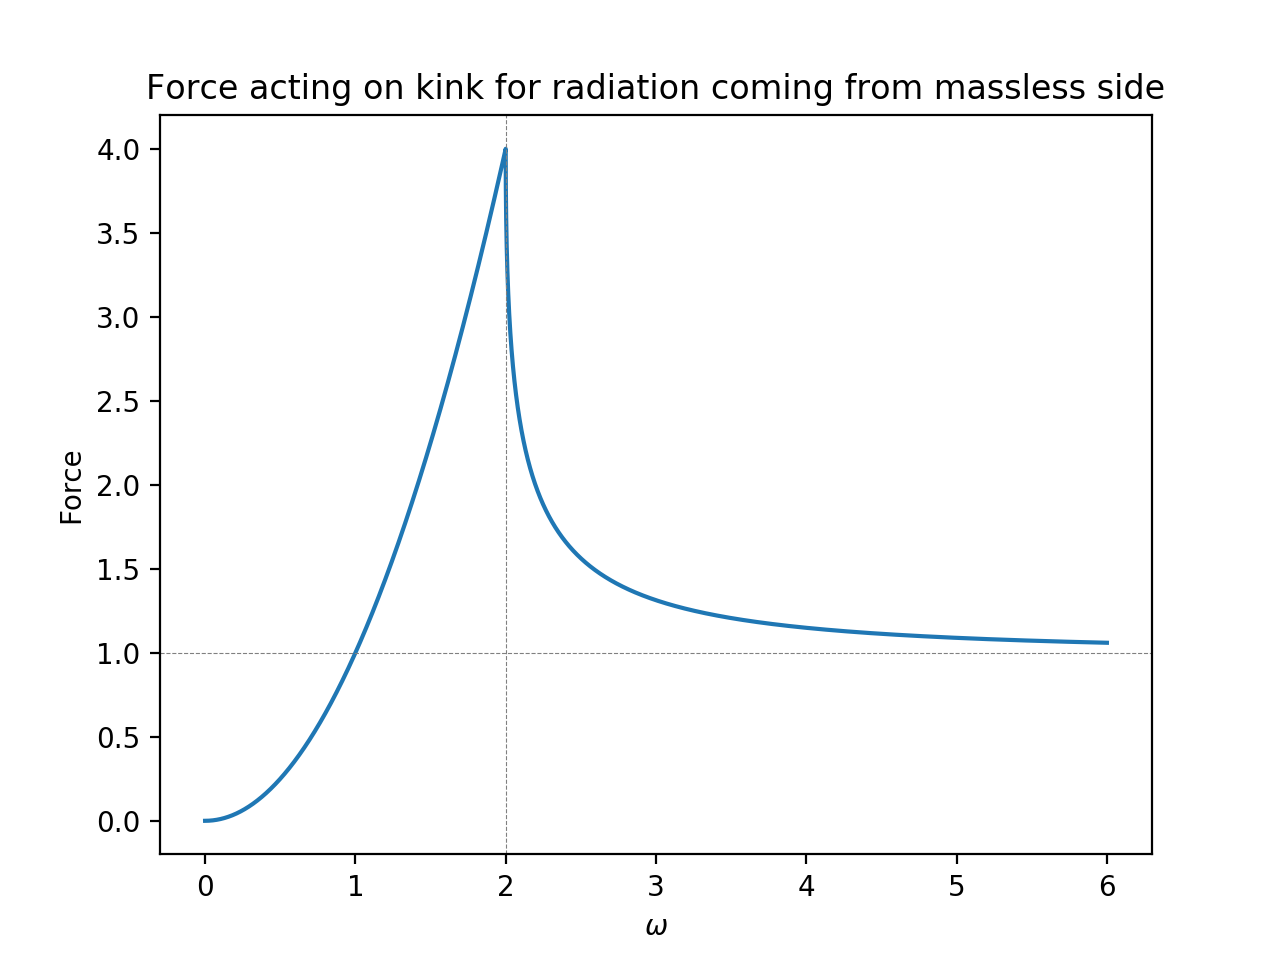
\includegraphics[width=0.4\textwidth]{force_left.png}
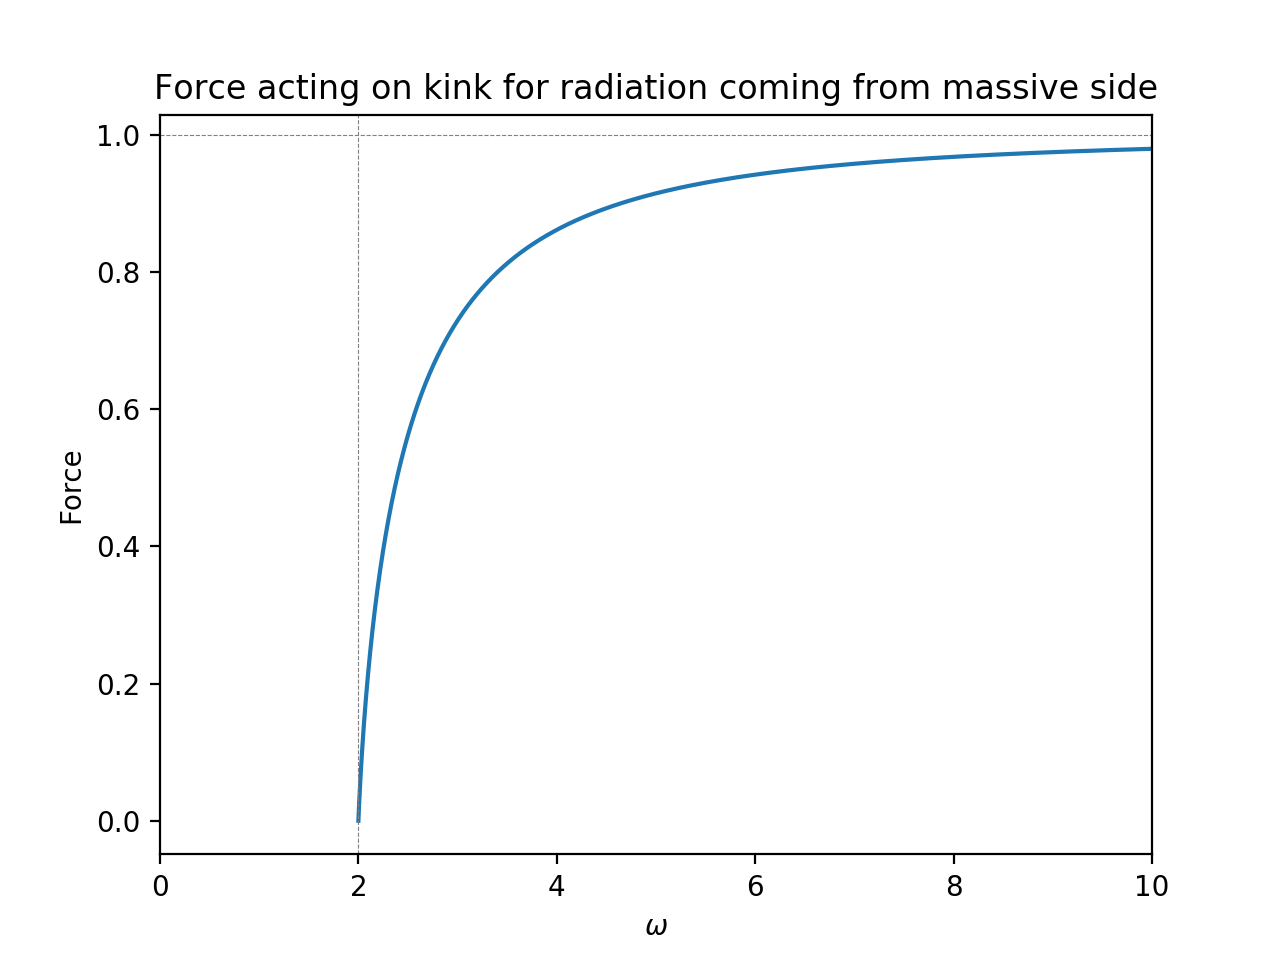
\includegraphics[width=0.4\textwidth]{force_right.png}
\captionof{figure}{Plots showing the strength of force acting on the kink from incident radiation coming from the massive and massless sides as a function of frequency} \label{force_left}
\end{figure}
Now we repeat the calculation for a plane wave with frequency $\omega$ coming from the massive side of the kink. In this case, since the wave starts in the region where $\omega^2 = k^2 + m^2$, waves with $\omega < 2$ are forbidden so $\alpha$ is always real here. \par
We propose a field profile containing reflected and transmitted waves
\begin{align}
\xi_\textup{left} &= T e^{i\omega (t+x)}\\
\xi_\textup{right} &= e^{-i\left( \omega t + \sqrt{\omega^2-4} x \right )} + Re^{-i\left( \omega t - \sqrt{\omega^2-4} x \right )} .
\end{align}
Matching boundary conditions gives us
\begin{equation}
R = \frac{\alpha-1}{\alpha+1},\; T = \frac{2\alpha}{\alpha+1}.
\end{equation}
Again in the limit of large $\omega$, $R \rightarrow 0$ and $T \rightarrow 1$, so the kink becomes transparent. The time-averaged momentum densities are
\begin{align}
 \left \langle \mathcal{P}_\textup{left} \right \rangle &= -\frac{1}{2}\omega^2 T^2 \\
 \left \langle \mathcal{P}_\textup{right} \right \rangle &= \frac{1}{2}\omega^2\alpha \left( -1 + R^2 \right) 
\end{align}
and the total force acting on the kink is given by
\begin{equation}
F = \frac{1}{2} \omega^2 \left ( -\alpha^2(1 +R^2) + T^2 \right ) .
\end{equation}
Once the values of $R$ and $T$ are substituted in we get a final expression
\begin{equation}
F = \omega^2 \alpha^2 \frac{1-\alpha^2}{(1+\alpha)^2} .
\end{equation}
This is plotted in fig.~\ref{force_left}. In both cases the overall force on the kink is positive, supporting the results from our numerical models. A notable feature is that as the frequency of radiation becomes large, the force exerted on the kink from either side tends to 1. This means that, regardless of the direction of incidence, radiation hitting a kink with high frequency will push the kink in the same direction with approximately the same force. We have set the amplitude of the incident radiation to be 1 in all cases here. Including amplitude would add a multiplicative $\mathcal{A}^2$ dependence to all of our force calculations here. This means that for large $\omega$, the strength of force acting on the kink is independent of $\omega$ and tends towards $F = \mathcal{A}^2$. 

\subsubsection{Averaging Out Background Radiation} \label{avg_out}
We now take a different approach to understanding the physics taking place here,  adding in a general radiation term to the field and averaging it out in order to gain a broad understanding of the effective potential felt by a kink in the presence of small background radiation. We start in the same way as in \textsection \ref{pert_theory}, by expressing the field in terms of a kink term $\varphi$ and a small radiation term $\xi$, assuming that $\xi \ll \varphi$. We also make the further assumption that the average value $\left \langle\xi\right \rangle$ is 0 and that $\left \langle\xi ^ 2\right \rangle > 0$ and examine the effect of $\xi$ on the potential $V(\varphi+\xi)$. Taylor expanding the potential gives:
\begin{equation}
V\left ( \varphi+\xi \right ) = V\left ( \varphi \right ) + \xi V'\left ( \varphi \right ) + \frac{\xi^2}{2}V''\left ( \varphi \right ) + \mathcal{O}(\xi^3).
\end{equation}
The Lagrangian for the field as a whole (eqn.~\ref{lagrangian}) becomes
\begin{equation}
\mathcal{L} = \frac{1}{2} \partial_\mu \varphi \partial^\mu \varphi + \partial_\mu \varphi \partial^\mu \xi + \frac{1}{2} \partial_\mu \xi\partial^\mu \xi- V\left ( \varphi \right ) + \xi V'\left ( \varphi \right ) + \frac{\xi^2}{2}V''\left ( \varphi \right ) + \mathcal{O}(\xi^3).
\end{equation} 
Now we take the average of the radiative field term, in order to look only at the behaviour of $\varphi$. The term proportional to $\xi$ vanishes due to the assumption made above. Similarly $\left \langle \partial^\mu \xi\right \rangle = 0$ for a wave, so we may discard the second term in $\mathcal{L}$. The term $ \frac{1}{2} \partial_\mu \xi\partial^\mu \xi$ does not depend on $\varphi$ at all so contributes a total shift to the Lagrangian, leaving the dynamics of $\varphi$ unaffected and so may be discarded. Thus we are left with the following expression, accurate to second order in $\xi$ 
\begin{equation}
\mathcal{L}_{\textup{eff}} = \frac{1}{2} \partial_\mu \varphi \partial^\mu \varphi - V\left ( \varphi \right ) - \frac{\left \langle \xi^2 \right \rangle}{2}V''\left ( \varphi \right ) .
\end{equation} 
This is equivalent to looking at a field $\varphi$ with an effective potential defined by
\begin{equation}
V_\textup{eff} = V\left ( \varphi \right ) + \frac{\left \langle \xi^2 \right \rangle}{2}V''\left ( \varphi \right ) 
\end{equation}
with
\begin{align}
V(\varphi) &= \frac{1}{2} \varphi \left ( 1- \varphi^2 \right )^2, \; \;V''(\varphi) = 6\varphi^2 - 30\varphi^4 + 28\varphi^6.
\end{align}
\begin{wrapfigure}{r}{0.45\textwidth}
\centering
 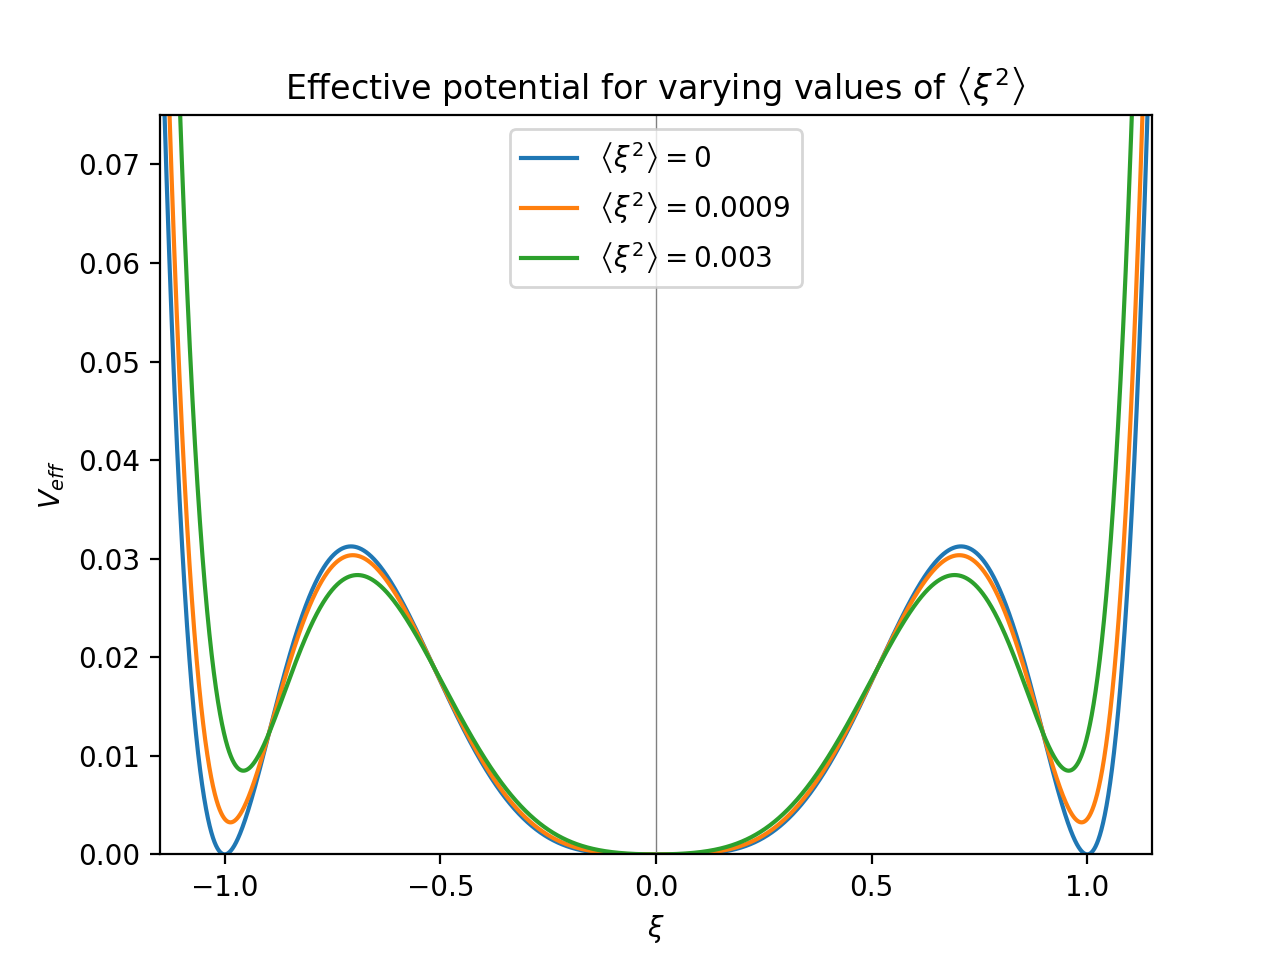
\includegraphics[width=0.45\textwidth]{potential_averaged.png}
 \captionof{figure}{Effective potential for $\left \langle \xi^2 \right \rangle = 0$, 0.003 and 0.0009.} \label{potential_averaged}
\end{wrapfigure}
Note that we have not said anything about the profile of $\xi$ other than that it is small when compared to $\varphi$ and has a wave-like shape, ensuring that $\xi$ and $\partial \xi$ average to 0. Figure \ref{potential_averaged} shows the effect of introducing a small $\left \langle \xi^2 \right \rangle$ term to the effective potential. As can be seen, averaging out radiation breaks the degeneracy of the ground state. The $\varphi = 0$ ground state becomes the global minimum, since $V''(0) = 0$, but the $\varphi = \pm1$ states both now have nonzero energy (as well as having the position of the minimum displaced slightly).\par
If we assume that the value of $\left \langle \xi^2 \right \rangle$ is small enough that the position of the minima at $\xi = \pm 1$ is not significantly affected, we can approximate the shift in energy of these two ground states using $V(\pm1) = 0$ and $V''(\pm 1) = 4 $.
\begin{equation}
V_{\textup{eff}}(\pm1) = 2 \left \langle \xi^2 \right \rangle.
\end{equation}
This shift in the energy of each vacuum will introduce a force that accelerates kinks to the right and anti-kinks to the left, eventually placing the whole system into the $\phi = 0$ ground state. The force acting on a kink can be calculated using the fact that the vacuum on the left of the kink has zero energy density, but the vacuum on the right has energy density $2 \left \langle \xi^2 \right \rangle$. This means that sliding the kink uniformly towards the side with $\phi = 1$ will remove a region of positive energy density and create a region of zero energy density. Using $F = \frac{\drv E}{\drv x}$, and treating the kink as a solid object with position $x$ we derive the expression for the force
\begin{equation}
F = 2\left \langle \xi^2 \right \rangle.
\end{equation}
We can compare this to the example $\xi = \mathcal{A}\sin( - \omega t \pm k x)$ that we used in section \ref{pert_theory}. For a wave with this profile $ \left \langle \xi^2 \right \rangle = \frac{1}{2}\mathcal{A}^2$ so the overall force acting on the kink becomes
\begin{equation}
F = \mathcal{A}^2.
\end{equation}
This matches up with the results we got in the previous section in the limit of large $\omega$, where the kink becomes transparent. Additionally, in this limit $\sqrt{\omega^2 - 4} \simeq \omega$ so the wavenumber of the radiation is similar on the massless and massive sides of the kink. This means that $\xi = \mathcal{A}\sin( - \omega t \pm k x)$ is a valid solution for the radiation field on both sides of the kink, since the values of $\omega$ and $k$ on either side become identical.

\section{Conclusion}
We have investigated the dynamics of kinks in $\phi^8$ theory, where on one side the field is massive and on the other the field is massless, predicting that an interacting kink and anti-kink should have an attractive force between them that scales with the fourth power of the separation. These interactions were numerically simulated, finding excellent agreement with theory when the kinks are well separated. However our models became less accurate as the kinks got closer together, with the force appearing to be weaker than predicted. This breakdown was expected, since our analytic results were based on the assumption that the kinks were well separated.\par
The primary difficulty encountered in numerically simulating the interacting kinks was in initialising the field into an appropriate configuration, since the results had an extreme sensitivity to imperfections in initial conditions. Any deviation from the ideal starting point introduced radiation into the system. We found that the sensitivity of the kinks dynamics to radiation was due to the asymmetric nature of interaction between radiation and a kink. Any amount of radiation, coming from any direction would always have the effect of accelerating a kink towards the massive side. Furthermore we found that as the frequency of radiation is increased, the dynamics of the interaction become truly insensitive to the direction of incident radiation, exerting a force of the same strength and direction on the kink.\par
These results have interesting consequences when thinking about such systems that might exist in nature. In particular, it suggests that a field where such kinks manifest, perhaps as boundaries in higher than $1 + 1$ dimensional space, would only be able to contain stable kinks in the complete absence of any other disturbances to the field. Any radiation whatsoever would have the effect of accelerating kinks and anti-kinks towards one another, which would then annihilate, creating more radiation that would go on the affect other kinks in the same way. A discussion of this effect is given in \cite{Roma_czukiewicz_2017}.\par
There are a number of further steps that can be taken to better understand these phenomena. The most obvious next step would be to extend the discussion in \textsection \ref{rad-anal}. We have only looked at the interaction of kinks and radiation to first order, with the radiation as a small perturbation to the static field. Furthermore we approximated the background potential as a step function. Thus it would be worth looking at more accurate approximations for the background potential, in particular taking into account the region of space where $m^2 < 0$. Furthermore it would be worthwhile to look at higher order terms in the expansion of the field, as is done in \cite{rad_pressure}, where the interactions between radiation and kinks is examined in a number of potentials, including $\phi^4$. Since the interaction is fundamentally nonlinear, there will be frequency mixing effects taking place, such as second harmonic generation, that we have neglected by only expanding to first order. It is worth noting that \cite{rad_pressure} only examines theories where the mass on either side of the kink is the same, so the majority of effects observed here do not occur. Furthermore the forces acting on kinks in their treatment are largely due to higher order terms in the Taylor expansion, so we may expect them to be substantially weaker than the dominant effects found here with $\phi^8$ kinks.\par
Finally, another possible extension would be to quantise the field around the kink and examine the interactions between the kink and radiation in this context. The results from \textsection \ref{avg_out} suggest that it would be useful to examine the way this theory changes under renormalisation, potentially offering a deeper insight into the ways that theories of this type might manifest in real physical systems.



\bibliography{kinksbib}

 \renewcommand\thesection{}
 \renewcommand\thesubsection{\Alph{subsection}}
 \section{Appendix}
 \subsection{Verification of Accuracy of Numerical Methods}\label{tests}
 The validity of our numerical simulation is tested by inputting a test field. The field is allowed to propagate under the equations of motion as described in \textsection \ref{kink_kink_comp}. The momentum and energy-density is then calculated for each moment in time, and integrated across the whole of space using the trapezium rule. The initial field, $\phi$ and $\dot{\phi}$ are shown in fig.~\ref{test_field}, as well as the plots of total momentum and energy against time.\par
\begin{figure}
\centering
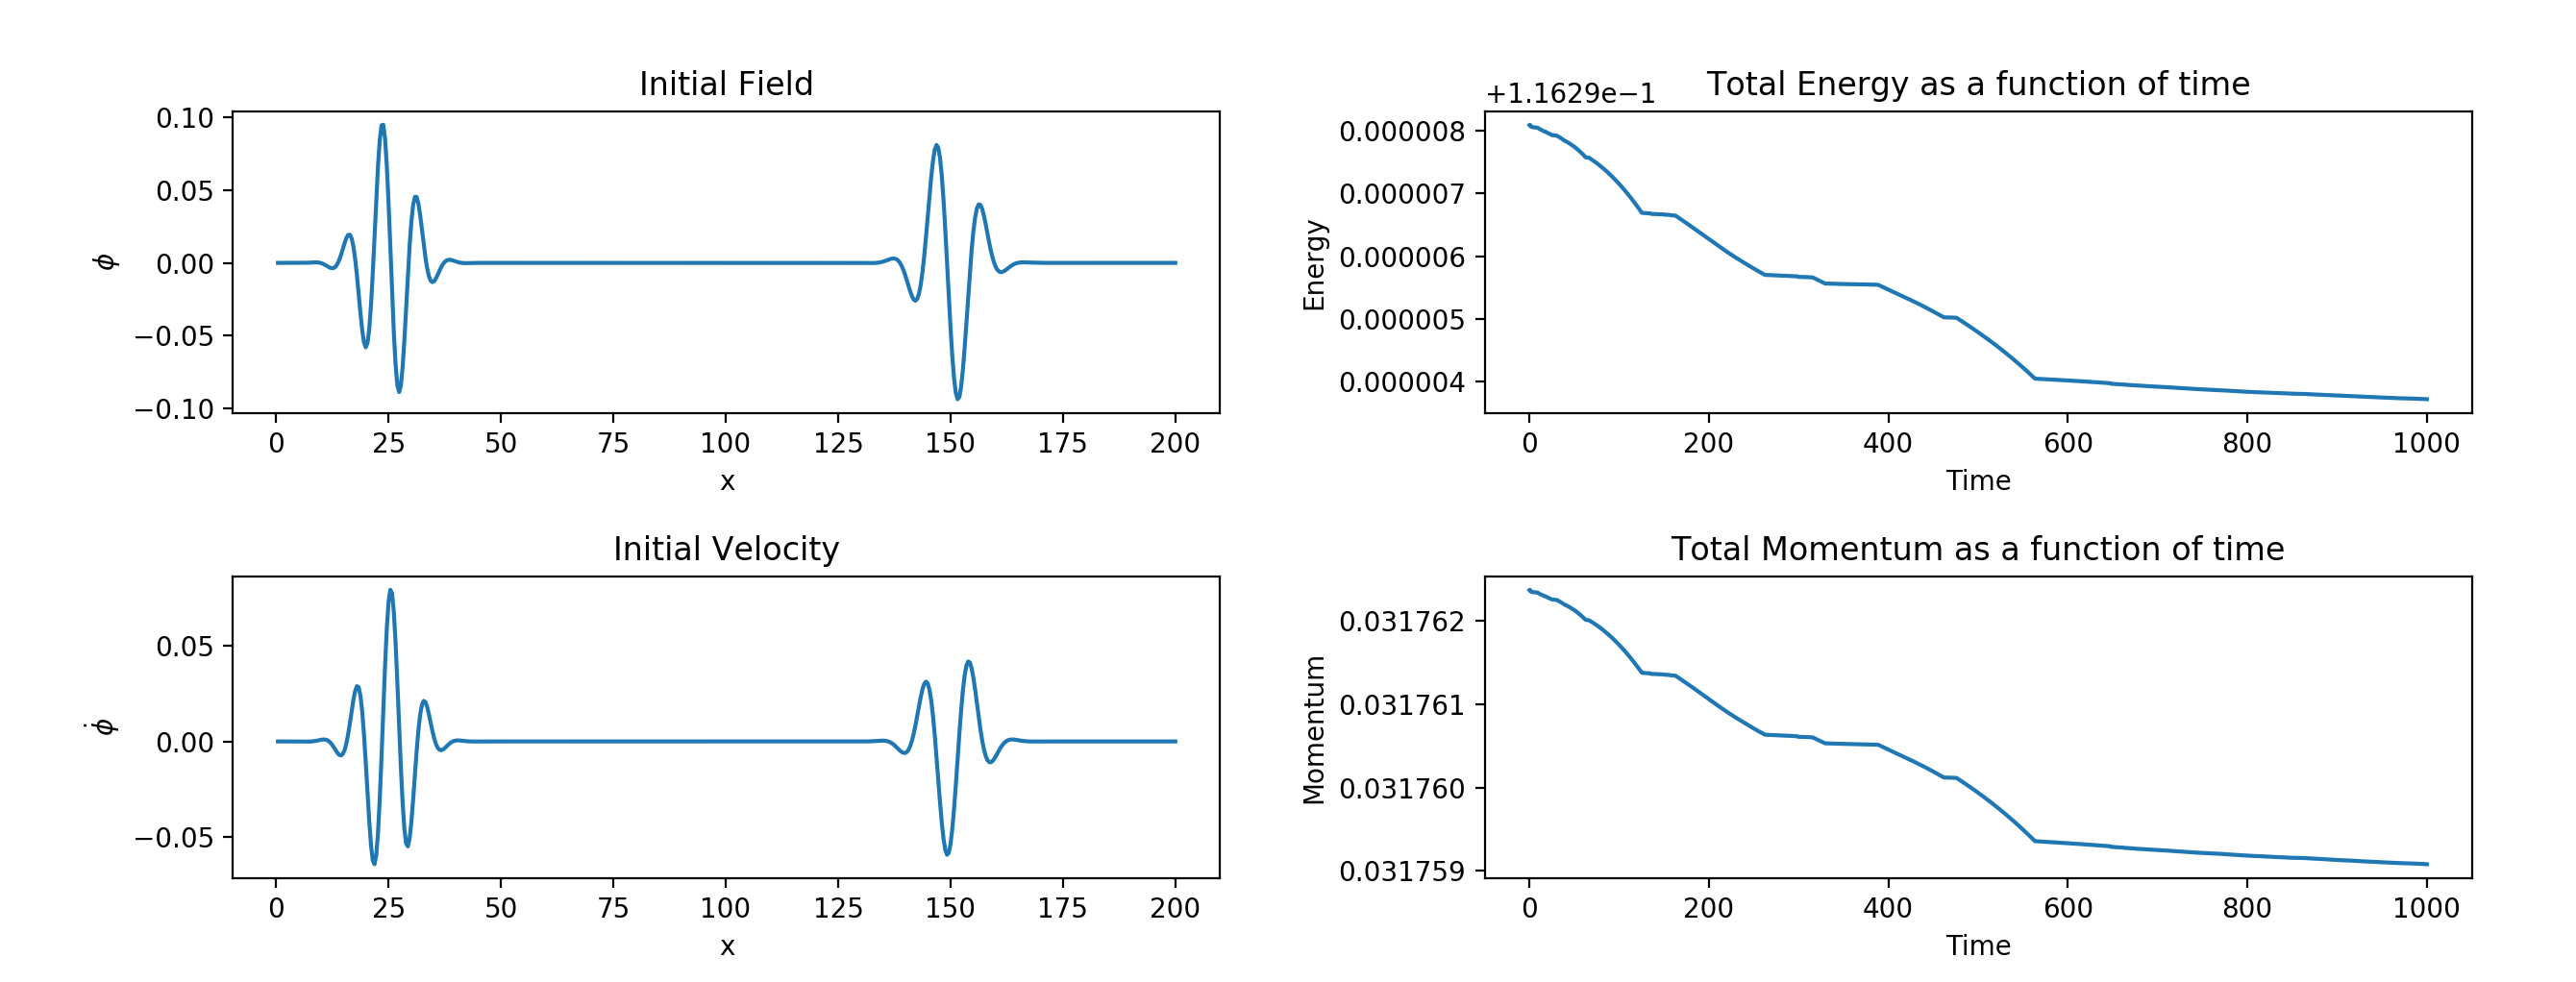
\includegraphics[width=0.8\textwidth]{test_field_energy.png}
\captionof{figure}{Plots showing the initial $\phi$ and $\dot{\phi}$ fields used, and the total energy and momentum calculated as a function of time} \label{test_field}
\end{figure}
Clearly neither the energy, nor the momentum are perfectly conserved, however the variation is extremely small (of the order $10^{-6}$). It is most likely that this variation is due to inaccuracies from numerically integrating the energy and momentum densities over the field. 


%\end{multicols}

\end{document} 